\documentclass[14pt,a4paper]{report}  %紙張設定
\usepackage{xeCJK}%中文字體模組
%\setCJKmainfont{標楷體} %設定中文字體
\setCJKmainfont{MoeStandardKai.ttf}
%\newfontfamily\sectionef{Times New Roman}%設定英文字體
\newfontfamily\sectionef{Nimbus Roman}
\usepackage{enumerate}
\usepackage{amsmath,amssymb}%數學公式、符號
\usepackage{amsfonts} %數學簍空的英文字
\usepackage{graphicx, subfigure}%圖形
\usepackage{fontawesome5} %引用icon
\usepackage{type1cm} %調整字體絕對大小
\usepackage{textpos} %設定文字絕對位置
\usepackage[top=2.5truecm,bottom=2.5truecm,
left=3truecm,right=2.5truecm]{geometry}
\usepackage{titlesec} %目錄標題設定模組
\usepackage{titletoc} %目錄內容設定模組
\usepackage{textcomp} %表格設定模組
\usepackage{multirow} %合併行
%\usepackage{multicol} %合併欄
\usepackage{CJK} %中文模組
\usepackage{CJKnumb} %中文數字模組
\usepackage{wallpaper} %浮水印
\usepackage{listings} %引用程式碼
\usepackage{hyperref} %引用url連結
\usepackage{setspace}
\usepackage{lscape}%設定橫式
\lstset{language=Python, %設定語言
		basicstyle=\fontsize{10pt}{2pt}\selectfont, %設定程式內文字體大小
		frame=lines,	%設定程式框架為線
}
%\usepackage{subcaption}%副圖標
\graphicspath{{./../images/}} %圖片預設讀取路徑
\usepackage{indentfirst} %設定開頭縮排模組
\renewcommand{\figurename}{\Large 圖.} %更改圖片標題名稱
\renewcommand{\tablename}{\Large 表.}
\renewcommand{\lstlistingname}{\Large 程式.} %設定程式標示名稱
\hoffset=-5mm %調整左右邊界
\voffset=-8mm %調整上下邊界
\setlength{\parindent}{3em}%設定首行行距縮排
\usepackage{appendix} %附錄
\usepackage{diagbox}%引用表格
\usepackage{multirow}%表格置中
%\usepackage{number line}
%=------------------更改標題內容----------------------=%
\titleformat{\chapter}[hang]{\center\sectionef\fontsize{20pt}{1pt}\bfseries}{\LARGE 第\CJKnumber{\thechapter}章}{1em}{}[]
\titleformat{\section}[hang]{\sectionef\fontsize{18pt}{2.5pt}\bfseries}{{\thesection}}{0.5em}{}[]
\titleformat{\subsection}[hang]{\sectionef\fontsize{18pt}{2.5pt}\bfseries}{{\thesubsection}}{1em}{}[]
%=------------------更改目錄內容-----------------------=%
\titlecontents{chapter}[11mm]{}{\sectionef\fontsize{18pt}{2.5pt}\bfseries\makebox[3.5em][l]
{第\CJKnumber{\thecontentslabel}章}}{}{\titlerule*[0.7pc]{.}\contentspage}
\titlecontents{section}[18mm]{}{\sectionef\LARGE\makebox[1.5em][l]
{\thecontentslabel}}{}{\titlerule*[0.7pc]{.}\contentspage}
\titlecontents{subsection}[4em]{}{\sectionef\Large\makebox[2.5em][l]{{\thecontentslabel}}}{}{\titlerule*[0.7pc]{.}\contentspage}
%=----------------------章節間距----------------------=%
\titlespacing*{\chapter} {0pt}{0pt}{18pt}
\titlespacing*{\section} {0pt}{12pt}{6pt}
\titlespacing*{\subsection} {0pt}{6pt}{6pt}
%=----------------------標題-------------------------=%             
\begin{document} %文件
\sectionef %設定英文字體啟用
\vspace{12em}
\begin{titlepage}%開頭
\begin{center}   %標題  
\makebox[1.5\width][s] %[s] 代表 Stretch the interword space in text across the entire width
{\fontsize{24pt}{2.5pt}國立虎尾科技大學}\\[18pt]
\makebox[1.5\width][s]
{\fontsize{24pt}{2.5pt}機械設計工程系}\\[18pt]
\sectionef\fontsize{24pt}{1em}\selectfont\textbf
{
\vspace{0.5em}
cd2023 2a-pj1ag1分組報告}\\[18pt]
%設定文字盒子 [方框寬度的1.5倍寬][對其方式為文字平均分分布於方框中]\\距離下方18pt
\vspace{1em} %下移
\fontsize{30pt}{1pt}\selectfont\textbf{網際手足球場景設計}\\
\vspace{1em}
\sectionef\fontsize{30pt}{1em}\selectfont\textbf
{
\vspace{0.5em}
Web-based Foosball Scene Design}
 \vspace{2em}
%=---------------------參與人員-----------------------=%             
\end{center}
\begin{flushleft}
\begin{LARGE}

\hspace{32mm}\makebox[5cm][s]
{指導教授:\quad 嚴\quad 家\quad 銘\quad 老\quad 師}\\[6pt]
\hspace{32mm}\makebox[5cm][s]
{班\qquad 級:\quad 四\quad 設\quad 二\quad 甲}\\[6pt]
\hspace{32mm}\makebox[5cm][s]
{學\qquad 生:\quad 第\quad 一\quad 位\quad(41023191)}
\\[6pt]
\hspace{32mm}\makebox[5cm][s]
{\hspace{36.5mm}第\quad 二\quad 位\quad(41023192)}\\[6pt]
\hspace{32mm}\makebox[5cm][s]
{\hspace{36.5mm}第\quad 三\quad 位\quad(41023193)}\\[6pt]
\hspace{32mm}\makebox[5cm][s]
{\hspace{36.5mm}第\quad 四\quad 位\quad(41023194)}\\[6pt]
\hspace{32mm}\makebox[5cm][s]
{\hspace{36.5mm}第\quad 五\quad 位\quad(41023195)}\\[6pt]
%設定文字盒子[寬度為5cm][對其方式為文字平均分分布於方框中]空白距離{36.5mm}\空白1em
\end{LARGE}
\end{flushleft}
\vspace{6em}
\fontsize{18pt}{2pt}\selectfont\centerline{\makebox[\width][s]
{中華民國\hspace{3em} 
112 \quad 年\quad 3\quad 月}}
\end{titlepage}
\newpage
%=---------------報告製作核可證明---------------------=%
 {\renewcommand\baselinestretch{1.4}\selectfont %設定以下行距
 {\begin{center}
    {\fontsize{20pt}{2.5pt} {國立虎尾科技大學 \qquad 機械設計工程系}\\[8pt]{分組報告製作合格認可證明}\\
    \hspace*{\fill} \\ %似enter鍵換行
    \par}
     \end{center}}
    {\begin{textblock}{60}(1.85,0.8)
    \noindent \fontsize{15pt}{16pt}\selectfont 分組報告製作修習學生\enspace:\quad
    {\begin{minipage}[t]{10em}\underline{四設二甲\enspace 41023191 第一位}\\ \underline{四設二甲\enspace 41023192\enspace 第二位}\\ \underline{四設二甲\enspace 41023193\enspace 第三位}\\ \underline{四設二甲\enspace 41023194\enspace 第四位}\\ \underline{四設二甲\enspace 41023195\enspace 第五位}\\ %下劃線符號指令
    \end{minipage}}
         \par} %結束指定行距
    {\renewcommand\baselinestretch{1.2}\selectfont %設定以下行距
    {\begin{textblock}{30}(1.8,4)
    \noindent \fontsize{16pt}{16pt}\selectfont 分組報告題目\enspace :網際手足球場景設計
    \hspace*{\fill} \\
    \hspace*{\fill} \\
    \noindent \fontsize{16pt}{16pt}\selectfont 經評量合格,特此證明
    \hspace*{\fill} \\
    \hspace*{\fill} \\
    \noindent \fontsize{16pt}{16pt} \makebox[6em][s]{評審委員}\enspace:\quad
    {\begin{minipage}[t]{6em} \underline{            }\\[16pt] \underline{            }\\[16pt] \underline{            }\\
    \end{minipage}}
    \end{textblock}}
    {\begin{textblock}{10}(1.8,9)
    {\begin{flushleft}
    \fontsize{16pt}{16pt}\selectfont \makebox[6em][s]{指導老師}\enspace:\quad \underline{            }\\[10pt]
    \hspace*{\fill} \\
    \fontsize{16pt}{2.5pt}\selectfont \makebox[12em][s]{中華民國一一二年}\hspace{2pt}
    \fontsize{16pt}{2.5pt}\selectfont\makebox[8em][s]{三月三十一日}
    \end{flushleft}}
    \end{textblock}}
    \end{textblock}}
     \par} %結束指定行距
     \newpage

%=------------------------摘要-----------------------=%
\renewcommand{\baselinestretch}{1.5} %設定行距
\pagenumbering{roman} %設定頁數為羅馬數字
\clearpage  %設定頁數開始編譯
\sectionef
\addcontentsline{toc}{chapter}{摘~~~要} %將摘要加入目錄
\begin{center}
\LARGE\textbf{摘~~要}\\
\end{center}
\begin{flushleft}
\fontsize{14pt}{20pt}\sectionef\hspace{12pt}\quad 由於矩陣計算、自動求導技術、開源開發環境、多核GPU運算硬體等這四大發展趨勢,促使AI領域快速發展,藉由這樣的契機,將實體機電系統透過虛擬化訓練提高訓練效率,再將訓練完的模型應用到實體上。\\[12pt]

\fontsize{14pt}{20pt}\sectionef\hspace{12pt}\quad 此專題是運用實體冰球對打機,將其導入CoppeliaSim模擬環境並給予對應設置,將其機電系統簡化並運用Open AI Gym進行訓練,找到適合此系統的演算法後,再到CoppeliaSim模擬環境中進行測試演算法在實際運用上的可行性。並嘗試透過架設伺服器將CoppeliaSim影像串流到網頁供使用者觀看或操控。\\[12pt]

\end{flushleft}
\begin{center}
\fontsize{14pt}{20pt}\selectfont 關鍵字: 類神經網路、強化學習、\sectionef CoppeliaSim、OpenAI Gym
\end{center}
\newpage
%=--------------------Abstract----------------------=%
\renewcommand{\baselinestretch}{1.5} %設定行距
\addcontentsline{toc}{chapter}{Abstract} %將摘要加入目錄
\begin{center}
\LARGE\textbf\sectionef{Abstract}\\
\begin{flushleft}
\fontsize{14pt}{16pt}\sectionef\hspace{12pt}\quad Due to the four major development trends of multidimensional arrays  computing, automatic differentiation, open source development environment, and multi-core GPUs computing hardware. The rapid development of the AI field has been promoted. In view of this development, the physical mechatronic systems can gain machine learning efficiency through their simulated virtual system training process. And afterwards to apply the trained model into real mechatronic systems.\\[12pt]

\fontsize{14pt}{16pt}\sectionef\hspace{12pt}\quad This project is to use the physical air hockey to play machine, introduce it into the CoppeliaSim simulation environment and give the corresponding settings, simplify its electromechanical system and use Open AI Gym for training, find an algorithm suitable for this system, and then perform it in the CoppeliaSim simulation environment Feasibility of testing algorithm in practical application. And try to stream CoppeliaSim images to web pages for users to watch or manipulate by setting up a server.\\
\end{flushleft}
\begin{center}
\fontsize{14pt}{16pt}\selectfont\sectionef Keyword:  nerual network、reinforcement learning、 CoppeliaSim、OpenAI Gym
\end{center}
\newpage
%=------------------------誌謝----------------------=%
\addcontentsline{toc}{chapter}{誌~~~謝}
\centerline\LARGE\textbf{誌~~謝}\\
\begin{flushleft}
\fontsize{14pt}{2.5pt}\hspace{12pt}\quad 在此鄭重感謝製作以及協助本分組報告完成的所有人員,首先向大三學長致謝,他們不辭辛勞解決我們的提問,甚至從來沒有不耐煩,總是貼心為我們找出最佳解答。再來是我們的分組組長,他給了我們全方位的支援,提供我們解決問題的方向和建議,給予開始接觸網際對戰遊戲的我們有個學習的方向,開會時也時不時向我們提出建議以及未來走向,同時也給了我們能自由摸索的空間及時間,最後是由本分組組員同心協力才得以完成本報告,特此感謝。
\end{flushleft}
\newpage
%=------------------------目錄----------------------=%
\renewcommand{\contentsname}{\centerline{\fontsize{18pt}{\baselineskip}\selectfont\textbf{目\quad 錄}}}
\tableofcontents  %目錄產生
\newpage
%=------------------圖表目錄產生----------------------=%
\renewcommand{\listfigurename}{\centerline{\fontsize{18pt}{\baselineskip}\selectfont\textbf{圖\quad 目\quad 錄 }}}
\newcommand{\loflabel}{圖} %定義\loflabel 文字為圖
\renewcommand{\numberline}[1]{\loflabel~#1\hspace*{0.5em}}
\listoffigures
%\newcommand{\captioname}{圖}
\newpage
\renewcommand{\listtablename}{\centerline{\fontsize{18pt}{\baselineskip}\selectfont\textbf{表\quad 目\quad 錄 }}}
\newcommand{\lotlabel}{表} %定義\lotlabel 文字為表
\renewcommand{\numberline}[1]{\lotlabel~#1\hspace*{0.5em}}
\listoftables

\end{center}
%=-------------------------內容----------------------=%
\chapter{前言}
\renewcommand{\baselinestretch}{10.0} %設定行距
\pagenumbering{arabic} %設定頁號阿拉伯數字
\setcounter{page}{1}  %設定頁數
\fontsize{14pt}{2.5pt}\sectionef
\section{研究動機}
機器學習與各領域結合的應用越來越廣泛,在機電系統採用強化學習是為了讓機電系統的控制達到最佳化。本專題以實體的冰球機,之機電系統作為訓練模型,將實體機器轉移到虛擬環境,進行模擬,為了找到適合的訓練參數,因此將模型簡化後再進行測試各種參數的優劣,透過不斷的訓練來得到一個優化過的對打系統。\\

\begin{figure}[hbt!]
\begin{center}
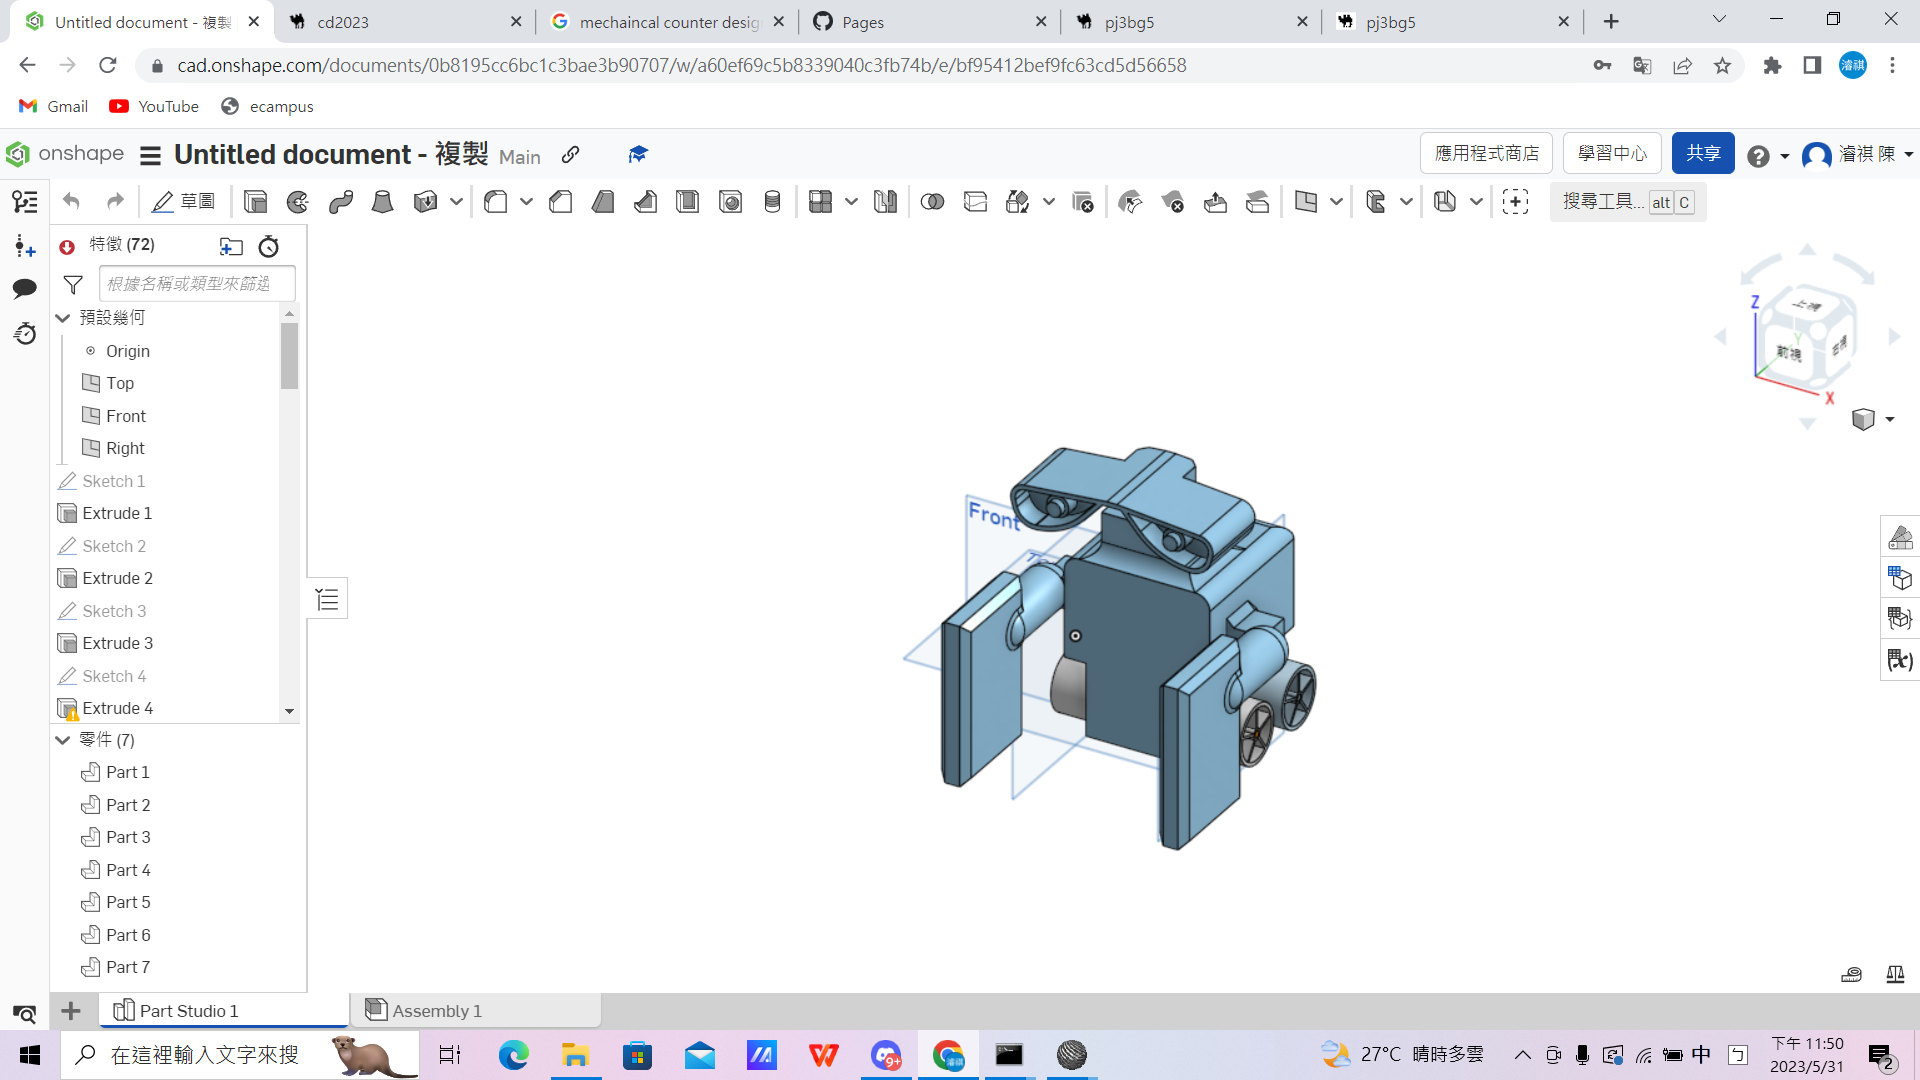
\includegraphics[angle=90,width=10cm]{11111}
\caption{\Large 實體的冰球機}\label{fig.冰球機}
\end{center}
\end{figure}
\begin{figure}[hbt!]
\begin{center}
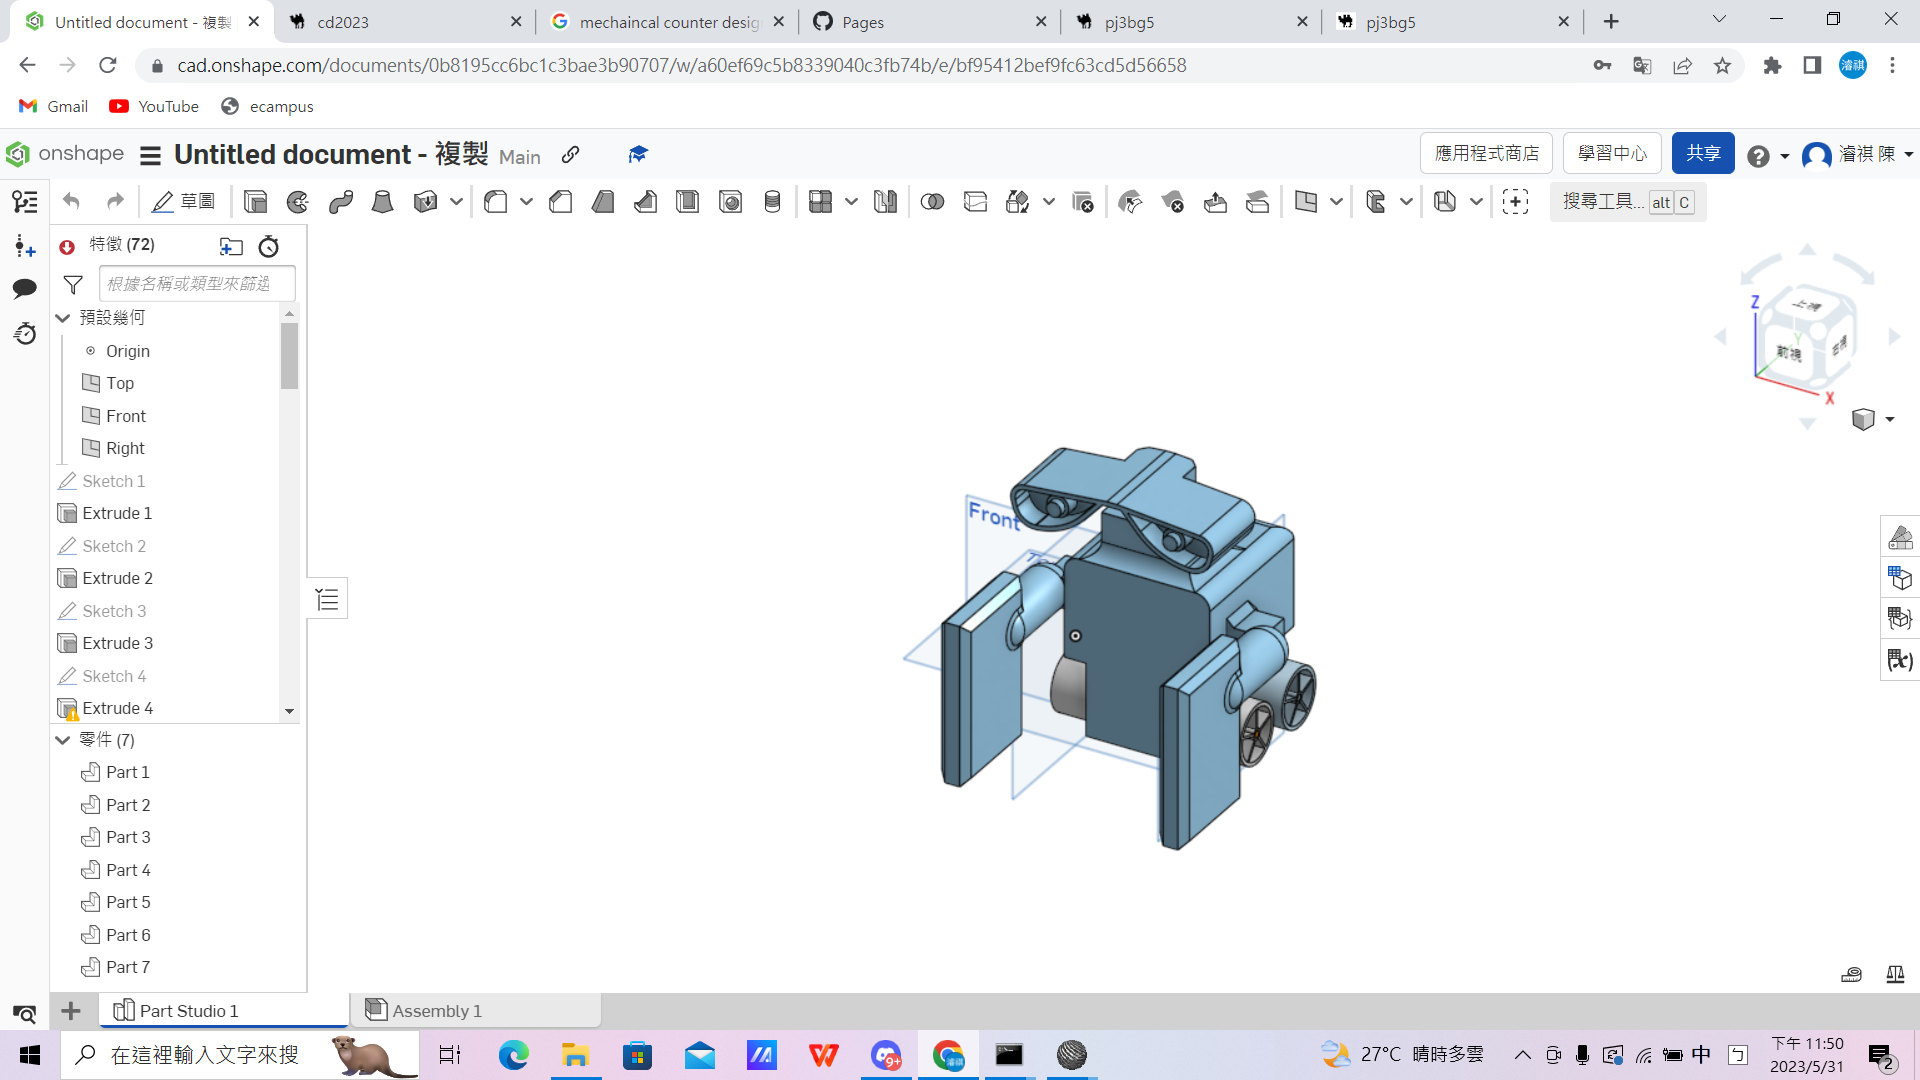
\includegraphics[angle=90,width=10cm]{11111}
\caption{\Large 虛擬環境簡化後的冰球機}\label{fig.模擬冰球機}
\end{center}
\end{figure}
\begin{figure}[hbt!]
\begin{center}
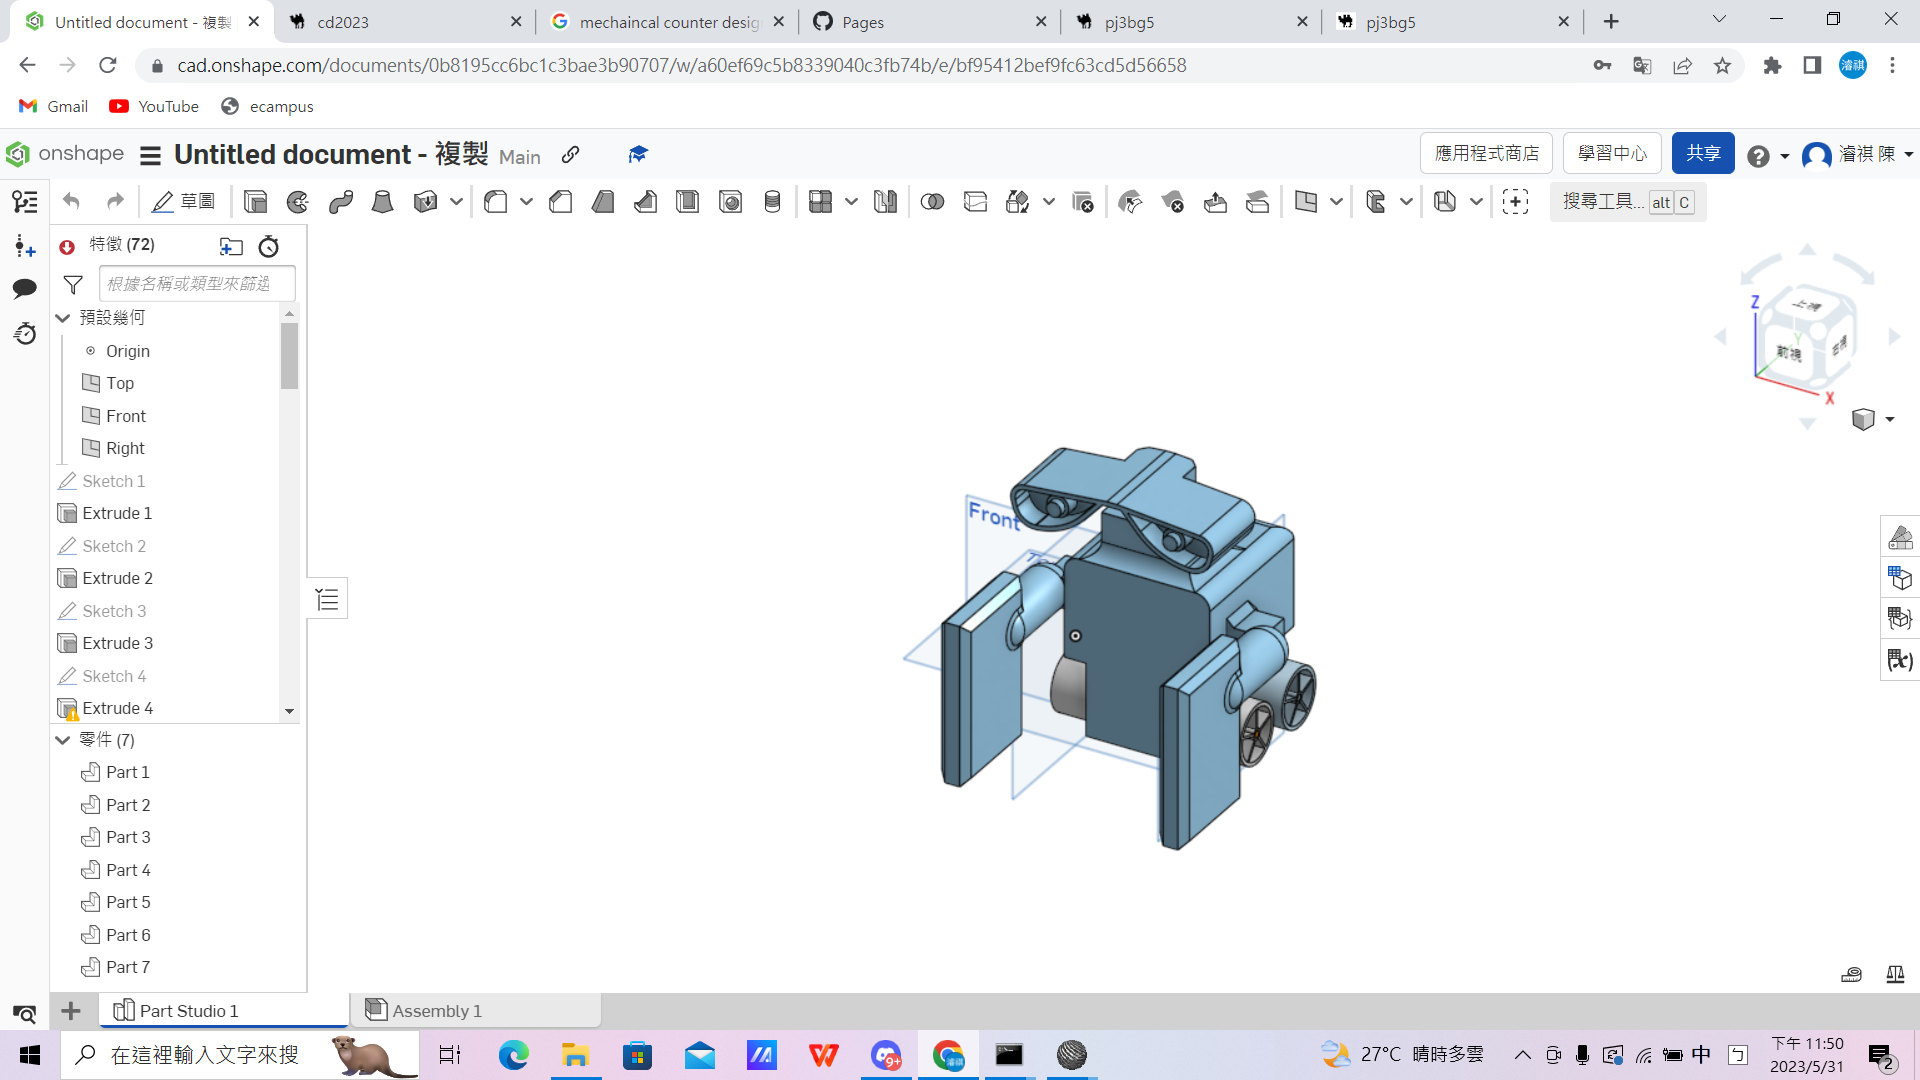
\includegraphics[height=8cm]{11111}
\caption{\Large Gym的Pong game}\label{fig.pong_gym}
\end{center}
\end{figure}


\section{研究目的與方法}
本研究分三大部分,第一運用OpenAI Gym裡內建編譯的ATARI 2600遊戲Pong-v0,來作為訓練環境,加上強化學習的理論,測試不同演算法參數以訓練出最佳化的對打系統,第二將整個簡化後冰球機導入CoppilaSim模擬環境並嘗試進行虛擬訓練,成為優化的對打機電系統。第三則是嘗試透過架設伺服器與虛擬環境結合。\\
 
透過簡化實體冰球機並導入虛擬環境,進行虛擬訓練,使用Gym的Pong當作對應的2D虛擬訓練環境,測試算法和訓練效果,篩選適合的算法與參數。\\

建置CoppilaSim模擬環境,嘗試將2D訓練概念套用到3D環境進行測試,加入電腦視覺與RemoteAPI,電腦視覺抓取球與擊錘的位置,透過RemoteAPI進行遠端控制,在3D環境測試算法可確保後續套用到實體機器上的可行性。\\
 
 再透過架設伺服器與虛擬環境結合:讓虛擬環境的影像透過網伺服器串流影像供使用者遠端進行操控虛擬環境的擊錘進行打球,或是提供多人進行觀看對打影像。
\begin{figure}[hbt!]
\begin{center}
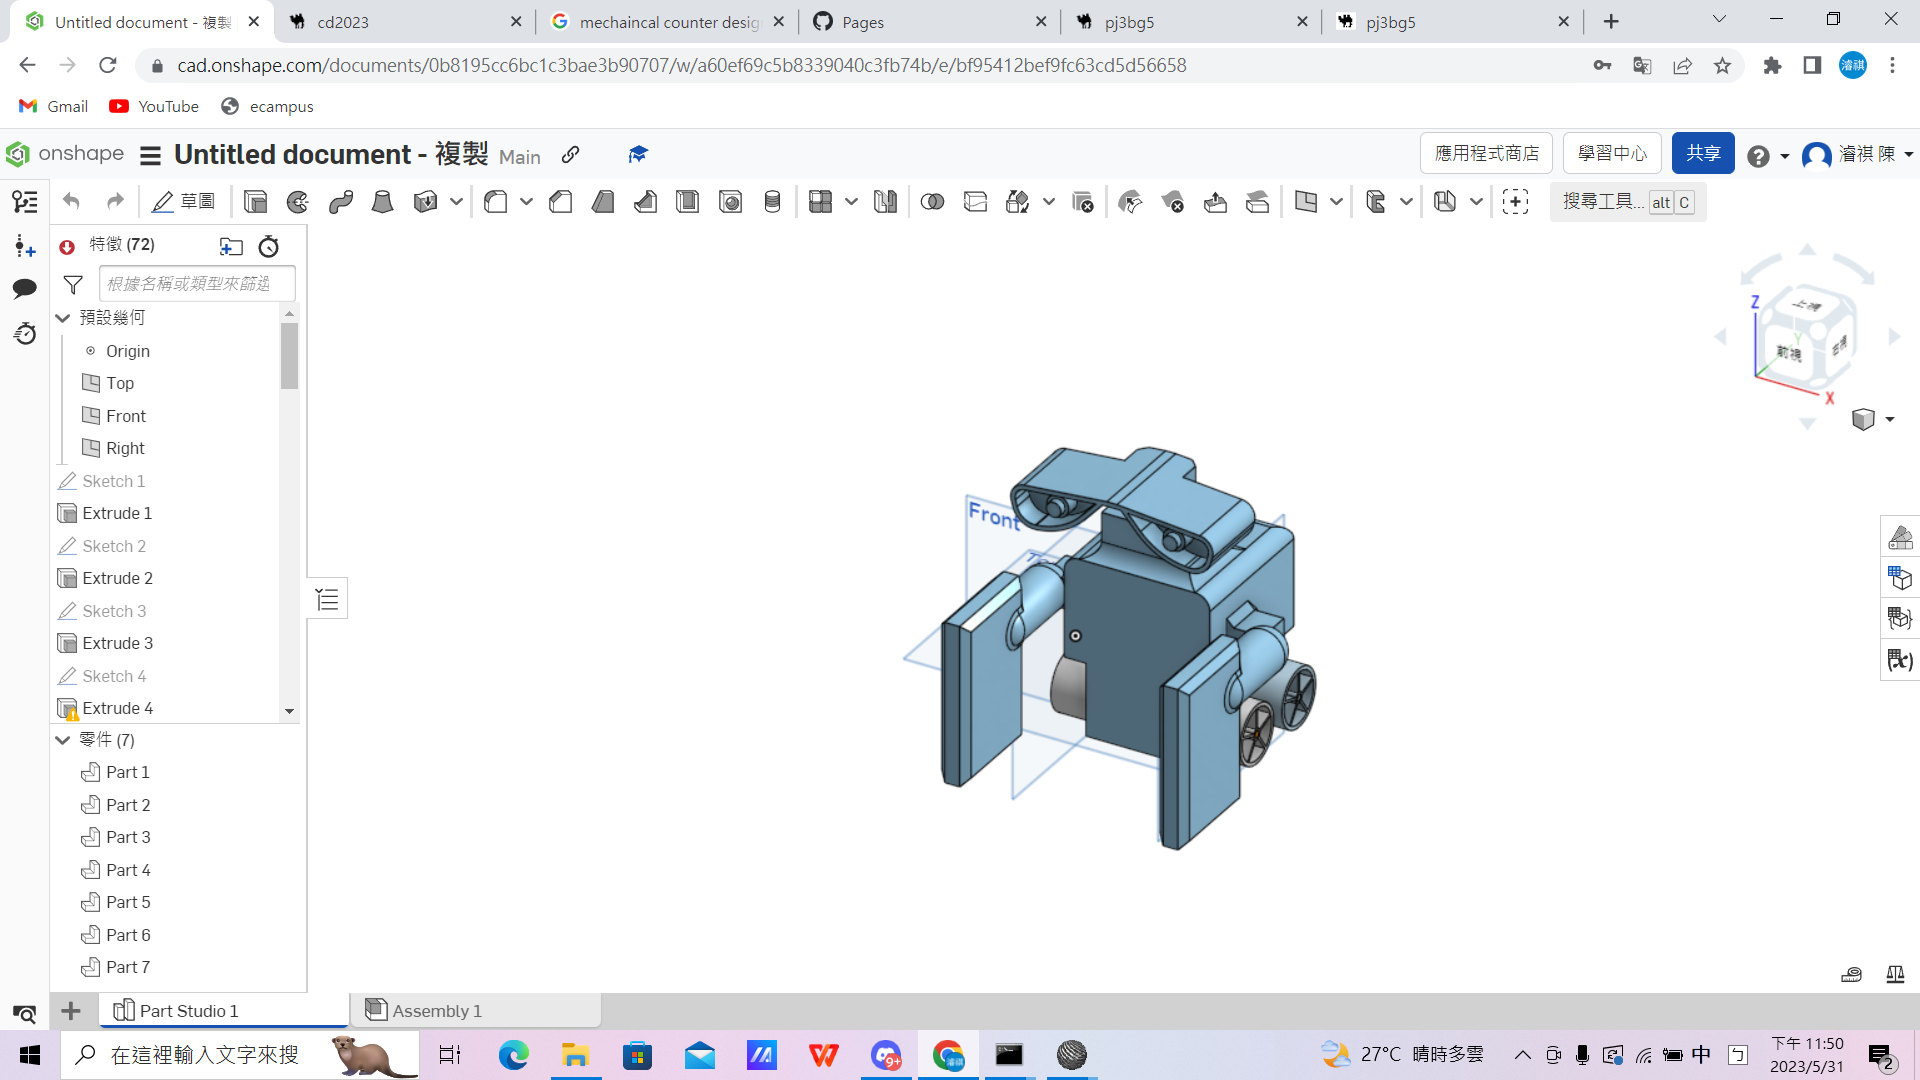
\includegraphics[width=15cm]{11111}
\caption{\Large 研究架構 }
\label{研究架構 }
\end{center}
\end{figure}
\section{未來展望}
此專題希望能利用現有完成的機械學習的算法,能發展成虛擬訓練,再將訓練完的機器學習應用到虛擬環境或是實體機電系統,並透過伺服器將影像串流提供玩家網頁介面進行遠端操控,同時提供多人觀看及時的比賽影像,將整個冰球機的控制和使用者間有更完善串聯,機電系統的部分達到最優化控制和虛實整合的應用。
\section{規則說明}
 Pong game 的遊戲規則簡單,透過擊錘將球打入對方球門即得一分,只要其中一方得21分就結束該局。擊錘只能沿單方向來回移動來進行防守和進攻。\\
遊戲規則如下:
\begin{enumerate}
\item 球打入敵方即得一分。
\item 擊錘只單一方向移動。
\item 最快贏得21分者獲勝,並結束該局遊戲。
\end{enumerate}

\renewcommand{\baselinestretch}{0.5} %設定行距

\chapter{機器學習}
\section{類神經網絡}
\begin{figure}[hbt!]
\begin{center}
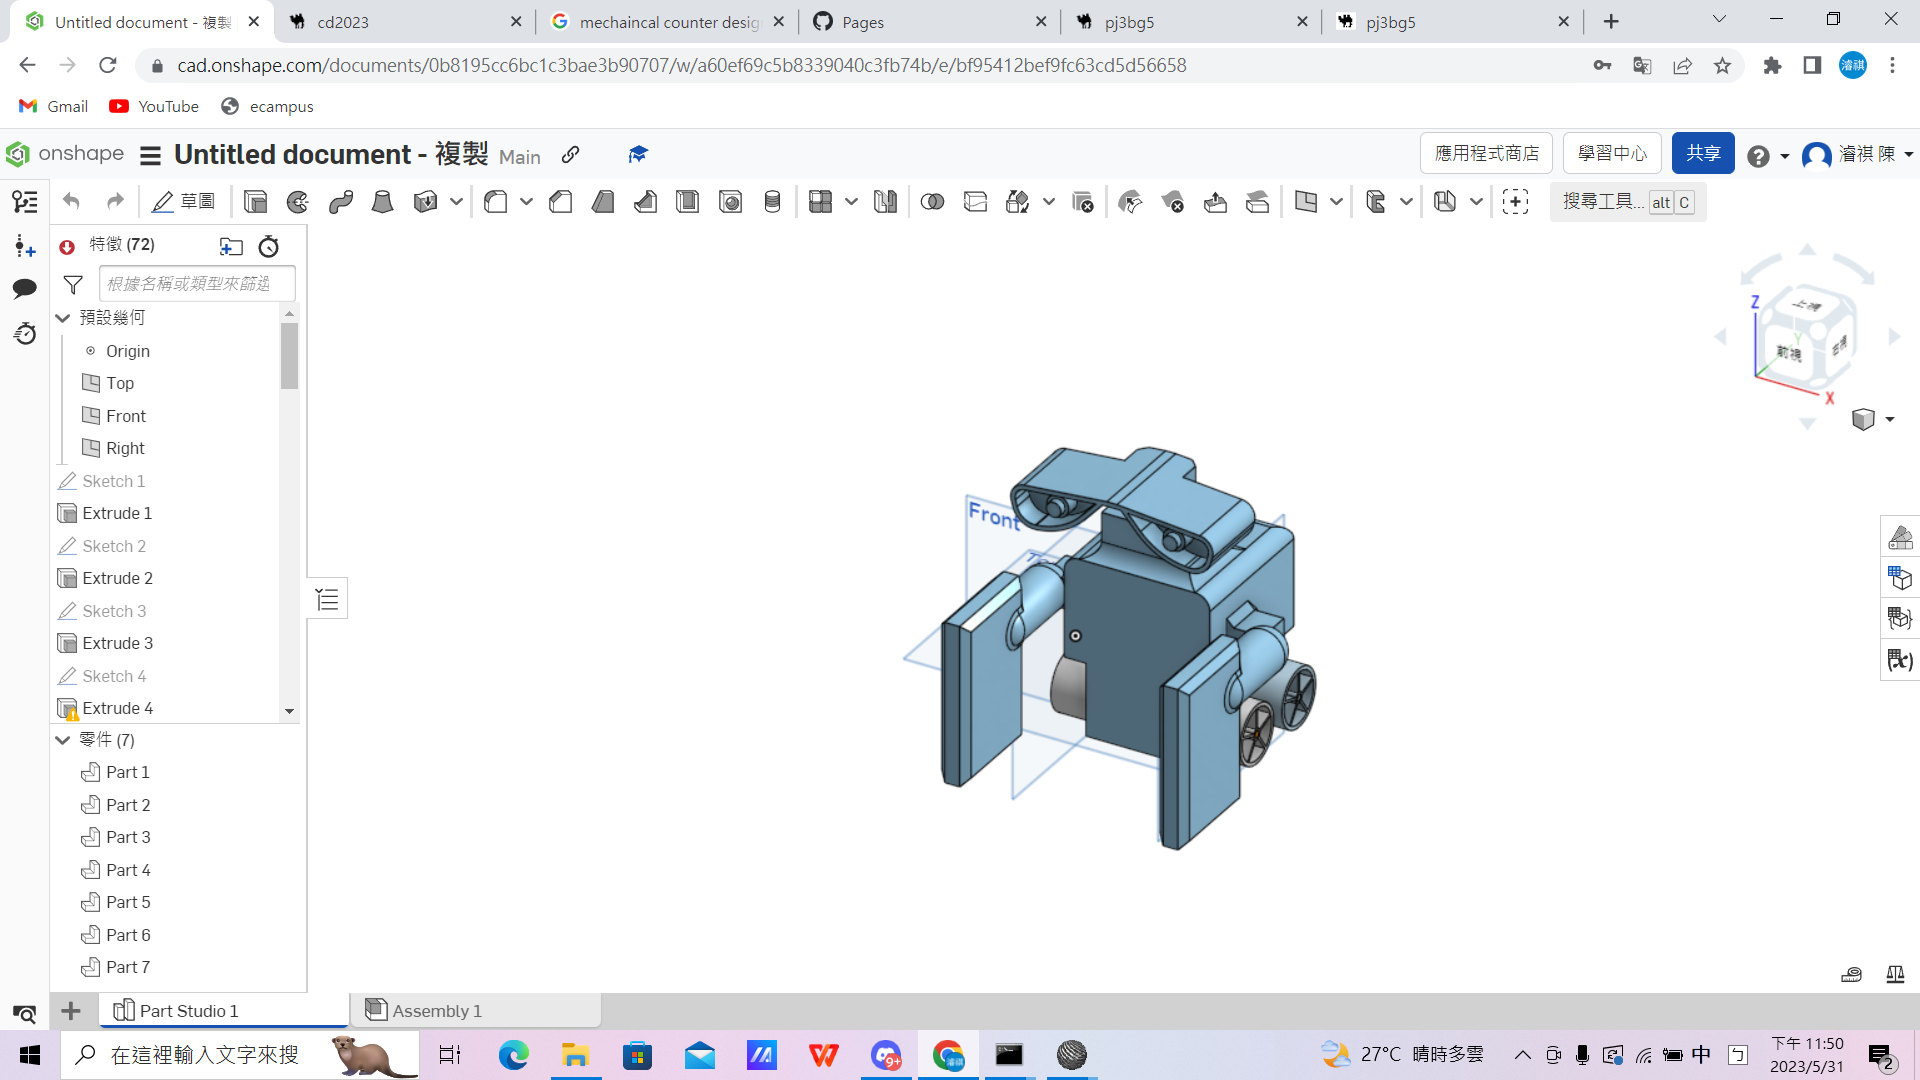
\includegraphics[width=16cm]{11111}
\caption{\Large 類神經網路架構}\label{類神經網路架構}
\end{center}
\end{figure}

 典型的類神經網路架構,如所示每一層的每一個神經元都會連接到下一層全部的神經元,對於每個神經元輸出會有不同的權重。\\

 神經元是AI系統中使用的數學模型,其行為與實際的大腦神經元運作方式相仿,模型以數字的方式表達,神經元間傳遞會有不同強度,而以數值的大小代表不同強度,這個數值我們稱為權重,對結果產生重要的影響。\\

 基礎的類神經網路架構主要由輸入層、隱藏層和輸出層這三部分組成,實際運用上還有更多樣更複雜的類神經網路架構,深度學習則是有更多的隱藏層,從意義上來說就是增加了類神經網路的深度。\\

 此外,如所示,資料由輸入層傳入,經過隱藏層運算和記憶,再由輸出層進行輸出,這種資料被傳遞的方式被稱為前饋輸入(feed-forward)。\\

 類神經網路架構有了記憶,就能進一步讓網路學習。當類神經網路接收資料並猜測答案,如果答案與實際答案不符、有落差或有錯誤的情況,它會回授並修改對每個神經元權重和偏差修正的程度,並嘗試調配各項數值來修正輸出的結果,讓結果的正確性提高,這樣的修正行為就被稱為反向傳播(back-propagation)。透過迭代方法進行反複試驗,模擬人們學習的行為,而每一次的迭代被稱為epoch,經過一定的迭帶次數後會透過反向傳播修正輸出的誤差,經過不斷執行的修正,最終類神經網路的學習會不斷進步並給出更好的答案,訓練時間長短取決於訓練項目的複雜程度。\\

 可以看到該神經網絡的輸出僅取決於互連的權重,還取決於神經元本身的偏差,雖然權重會影響啟動函數曲線的陡度,但是偏差會將發生變化的整個曲線,向右或向左,權重和偏差的選擇,決定了單個神經元的預測強度,而訓練類神經網絡使用的輸入數據可以來微調權重和偏差。\\

\newpage
\begin{figure}
\begin{center}
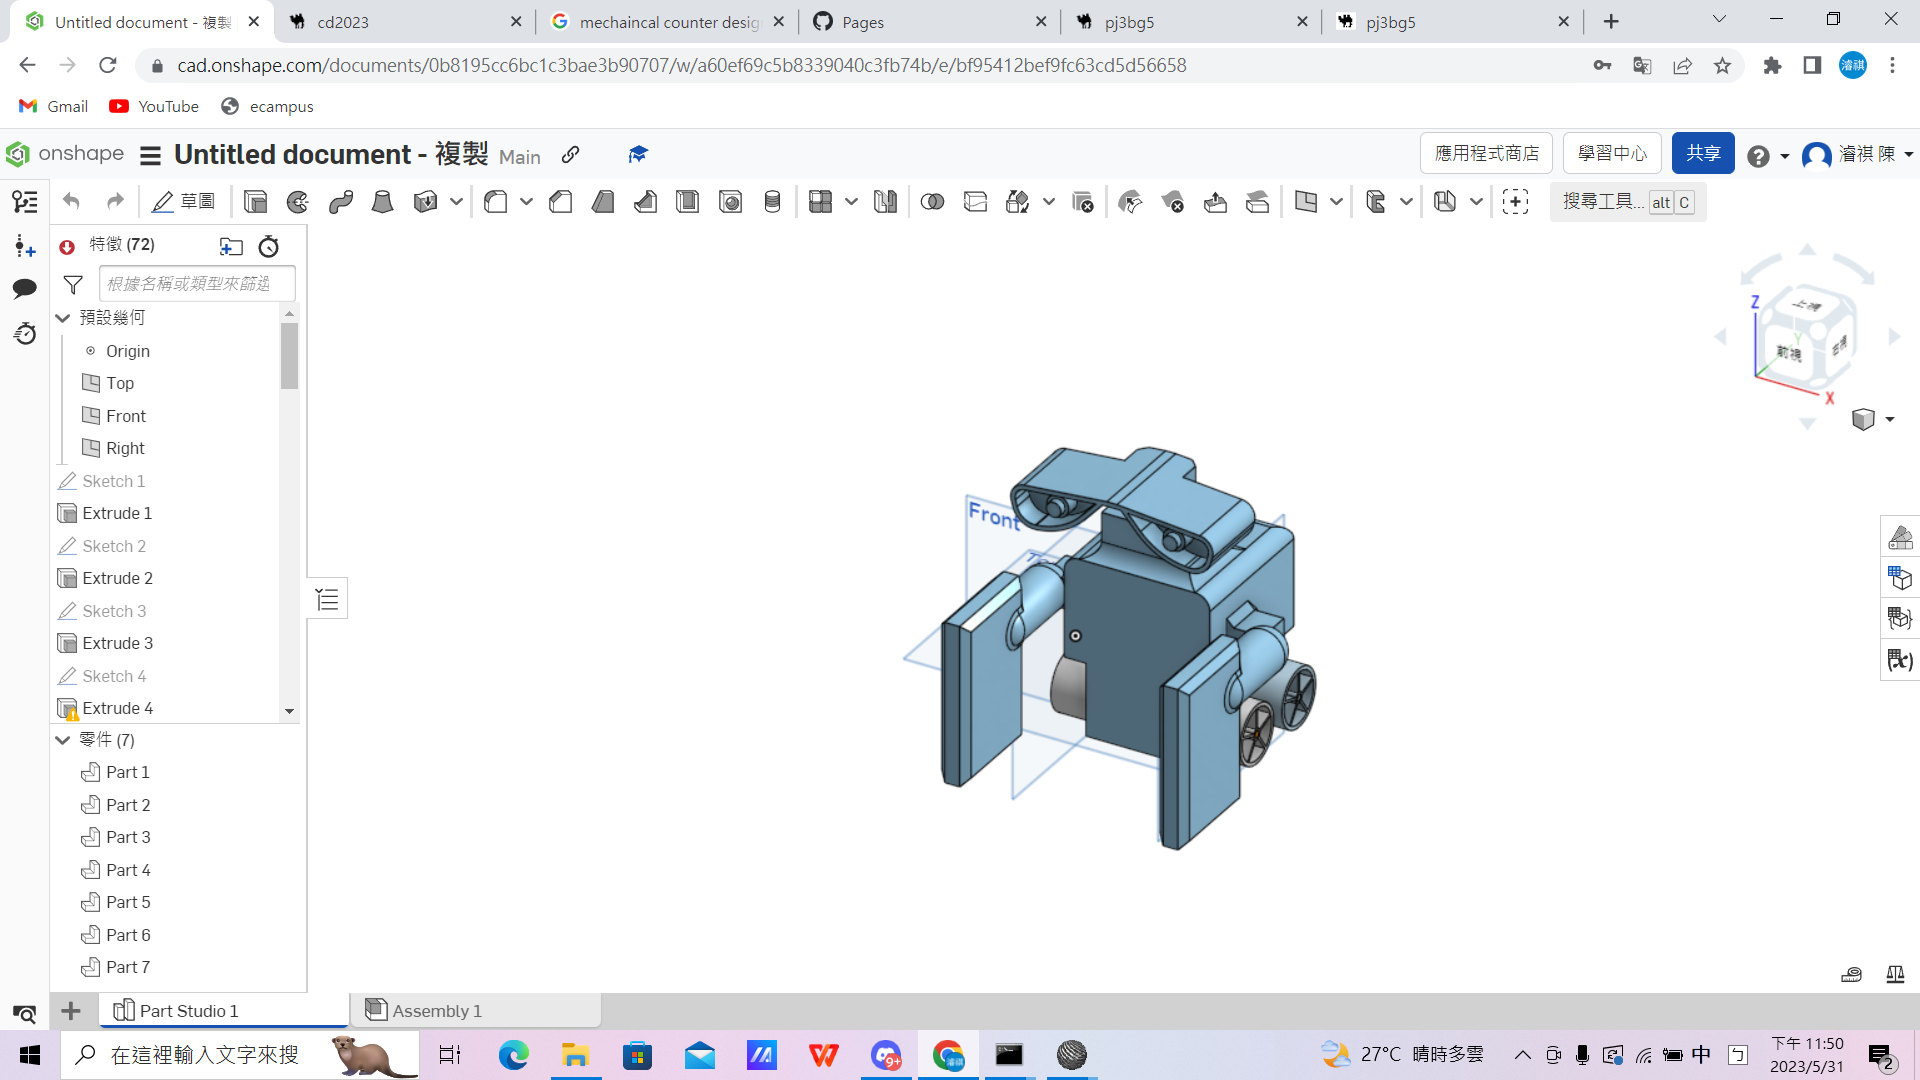
\includegraphics[width=16cm]{11111}
\caption{\Large 類神經網路關係}
\label{類神經網路關係}
\end{center}
\end{figure}
\subsection{啟動函數}
啟動函數是設計類神經網路的關鍵部分,如果不使用啟動函數,神經元的計算只會有線性組合,這樣的類神經網路缺乏活性而且記憶性差;啟動函數能讓神經元計算呈現非線性,讓類神經網路因為計算的非線性而提高整個網路的活性和記憶性。\\
以下介紹幾種較為常見的啟動函數及其特性:
\begin{itemize}
\\
%=----------Softmax Function----------=%
\item Softmax:\\
Softmax會計算每個事件分布的機率,適用多項目分類、其機率總合為1。以此專案為例,假設擊錘移動有向上移動、向下移動及不移動這三個決策選項,則這三個決策機率值總和為1。\\
$$S(x)=\frac{e^{x_i}}{\sum^k_{j=1}e^{x_i}}$$
%=----------Relu Function----------=%
\item ReLU Function:\\
ReLU Function方程式特性:若輸入值為負值,輸出值為0;若輸入值為正值,輸出則維持該輸入數值。ReLU計算方式簡單、收斂速度快,這是類神經網路最普遍拿來使用的啟動函數,因為可以解決梯度消散的問題,但須注意:起始值若設定到不易被激活範圍或是權重過渡所導致權重梯度為0就會造成神經元難以被激活。\\
\end{itemize}
$$f(x)=max(0,x)$$
$$if , x<0 , f(x)=0$$
$$else f(x)=x$$
\subsection{損失函數}
損失函數是類神經網路的另一個重要的部分,損失函數會將類神經網絡的結果與期望結果進行比較,且必須重複估算模型當前狀態的誤差;該函數可用於估計模型的損失,以便可以更新權重減少下次評估時的損失,下一節會有詳細說明,以下簡述幾種優化的方法:\\
\begin{itemize}
\item Gradient Descent\\
利用梯度的方式尋找最小值的位置,其特色可找到凸面error surface的絕對最小值,在非凸面error surface上找到相對最小值。其缺點是在非凸面error surface要避免被困在次優的局部最小值。
\item Batch gradient descent\\
用批次的方式計算訓練資料,整個資料集計算梯度只更新一次,因此計算和更新時會占用大量記憶體。整體效率較差、速度較緩慢。由 Gradient Descent 延伸出來的算法。其收斂行為與 Gradient Descent 相同。
\item Stochastic gradient descent\\
每次執行時會更新並消除誤差,有頻繁更新和變化大的特性,較不容易困在特定區域。由 Gradient Descent 延伸出來的算法。其收斂行為與 Gradient Descent 相同。
\item Mini-batch gradient descent\\
結合 Batch gradient descent 和 Stochastic gradient descent 的特點:批量計算和頻繁更新,所衍伸的算法。利用小批量的方式頻繁更新,並使收斂更穩定。其缺點:學習率挑選不易、預定義 threshold 無法適應數據集的特徵、對很少發生的特徵無法執行較大的更新、非凸面error surface要避免被困在次優的局部最小值等。
\item Gradient descent optimization algorithms\\
為了改善前面幾種算法而發展出來的優化算法。以下將列出數種優化算法。
\item Momentum\\
在梯度下降法加上動量的概念,會加速收斂到最小值並減少震盪。
\item Nesterov accelerated gradient\\
NAG,有感知能力的 Momentum:在坡度變陡時減速,避免衝過最小值所造成的震盪(為了修正到最小值,來回修正而產生的震盪)。
\item Adagrad\\
其學習率能適應參數:頻繁出現的特徵用較低的學習率,不經常出現的特徵則用較高的學習率,且無須手動調整學習率。其缺點是,學習率會急遽下降,最後會無限小,這算法就不再獲得知識。
\item Adadelta\\
為 Adagrad 的延伸,下降激進程度,學習率從更新規則中淘汰,不需設定預設學習率。
\item RMSprop\\
為了解決 Adagrad 學習率急劇下降的問題,學習率除以梯度平方的RMS,解決學習率無限小的情形。
\item Adam Function\\
結合了 Adagrad 和 RMSprop的優勢,有論文表示,在訓練速度方面有巨大性的提升,但在某些情況下,Adam實際上會找到比隨機梯度下降法更差的解決方法。以下是計算過程:\\
$$g_t=\delta_{\theta}f(\theta)$$
一次矩指數移動均線 :\\
$$m_t =\beta(m_{t-1})+(1-\beta_1)(\nabla{w_t})$$
$$\hat m_t=\frac{m_t}{1-\beta_1^t}$$
二次矩指數移動均線 :\\
$$v_t=\beta_2(v_t-1)+(1-\beta_2)(\nabla{w_t})^2$$
$$\hat{v_t}=\frac{v_t}{1-\beta_2^t}$$
因此,Adam Function:\\
$$\omega_{t-1}=\omega_t-\frac{\eta}{\sqrt{\hat{v_t}-\epsilon}}\hat{m_t}$$
\item AdaMax\\
與 Adam 相似,依靠$(u_t)$ 最大運算。
\item Nadam\\
結合 Adam 和 NAG ,應用先前參數執行兩次更新,一次更新參數一次更新梯度。
\item AMSGrad\\
改善 Adam 算法所導致收斂較差的情況(用指數平均會減少其影響),換用梯度平方最大值來做計算,並移除去偏差的步驟。是否有比 Adam 算法好仍有待觀察。
\item Gradient noise\\[6pt]
有助於訓練特別深且復雜的網絡,noise 可改善不良初始化的網路。
\item Mean Squared Error\\
他能告訴你一組點與回歸線接近的程度,透過獲取點與回歸線之距離(這些距離就是誤差)並對它們進行平方來做到這點,而平方是為了消除所有負號,也能讓更大的差異賦予更大的權重。\\
\vspace{8cm}
\newpage

\section{強化學習}
%=----------What is Reinforcement Learning?------------=%
強化學習(Reinforcement Learning,簡稱為RL)是通過agent(代理)與已知或未知的環境持續互動,不斷適應與學習,會得到正向或負面的回饋,對應到獎賞(reward)和懲罰(punishments)。考慮到agent與環境(environment)互動,進而決定要執行哪個動作,強化學習的學習模式是建立在獎賞與懲罰上。\\

強化學習與其他學習法不一樣的地方在於:不需要事先收集大量數據提供當作學習樣本,而是透過與環境互動,在環境下發生的狀態當作學習的資料來源,透過不斷嘗試使所得到的獎勵最大化。其他類型的機器學習大都需要給予特定資料且有明確的答案。\\

由於強化學習是建立在agent與環境互動上,因此許多參數進行運算,需要大量資訊來學習,並根據資訊採取行動。強化學習的環境可以是真實世界、2D或3D模擬世界的場景。強化學習的範圍很廣,因為環境的規模可能很大,且在環境中有多相關因素,影響著彼此。強化學習以獎勵的方式,促使學習結果趨近或達到目標結果。\\

\newpage

\chapter{訓練環境}
\section{OpenAI Gym}
 Gym 是用於開發和比較強化學習算法的工具包,他不對agent的結構做任何假設,並且與任何數據計算庫兼容,而可以用來制定強化學習的算法。這個環境具有共享的介面,使我們能用來編寫常規算法,也就能教導agents如何步行到玩遊戲。\\[6pt]

\section{Pong}
 取自 1977年發行的一款家用遊戲機ATARI 2600中的遊戲,內建於Gym,這是一個橫向的乒乓遊戲,左方是預設電腦玩家,右邊由使用者或是由訓練程式控制(圖.\ref{fig.pong})。在強化學習範例中,Pong與實體冰球機簡化後環境相似。\\
\begin{figure}[hbt!]
\begin{center}
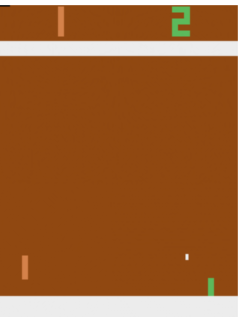
\includegraphics[height=8cm]{pong_gym}
\caption{\Large ATARI Pong}\label{fig.pong}
\end{center}
\end{figure} 

\newpage
\chapter{模擬環境}
%\renewcommand{\baselinestretch}{10.0} %設定行距
\section{模擬模型}
 在模擬的模型上,延用了學長設計的冰球機,並進行了部分的設計變更,將原本的人機對打更改為機器對打,且因為搭配深度強化學習的訓練,所以將兩邊的擊球器都僅保留X軸向(左右)移動,而冰球則是使用原本設計。多虧了學長們所設計的冰球機模型,讓我們在運作上有問題時可以直接發問,設計變更的地方也可以快速完成。\\
\begin{figure}[hbt!]
\center
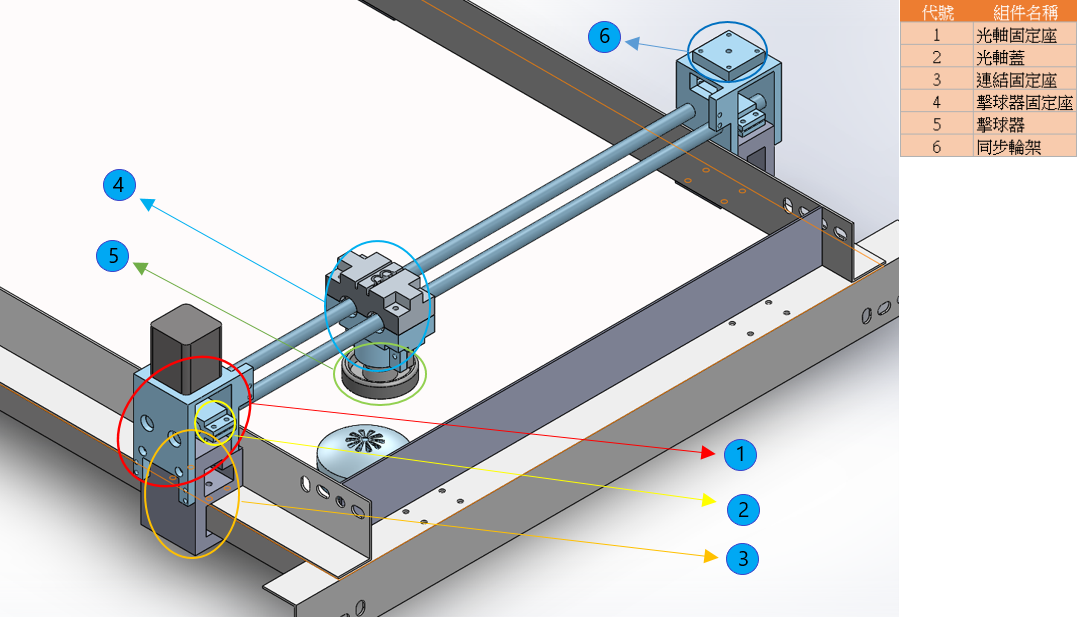
\includegraphics[width=13cm]{model}
\caption{\Large 組合圖}
\label{model}
\end{figure}

\qquad 將原本Y軸移動機構移除,並將其改為固定在特定位置上,此固定座設計是取代原本鎖在光軸固定坐上的(圖.\ref{model} 代號 1)Y軸皮帶固定座(圖.\ref{axialseat}),並使光軸固定座可以通過連結固定做鎖固於桌面,如(圖.\ref{connectSeat})。\\

\begin{figure}[hbt!]
\center
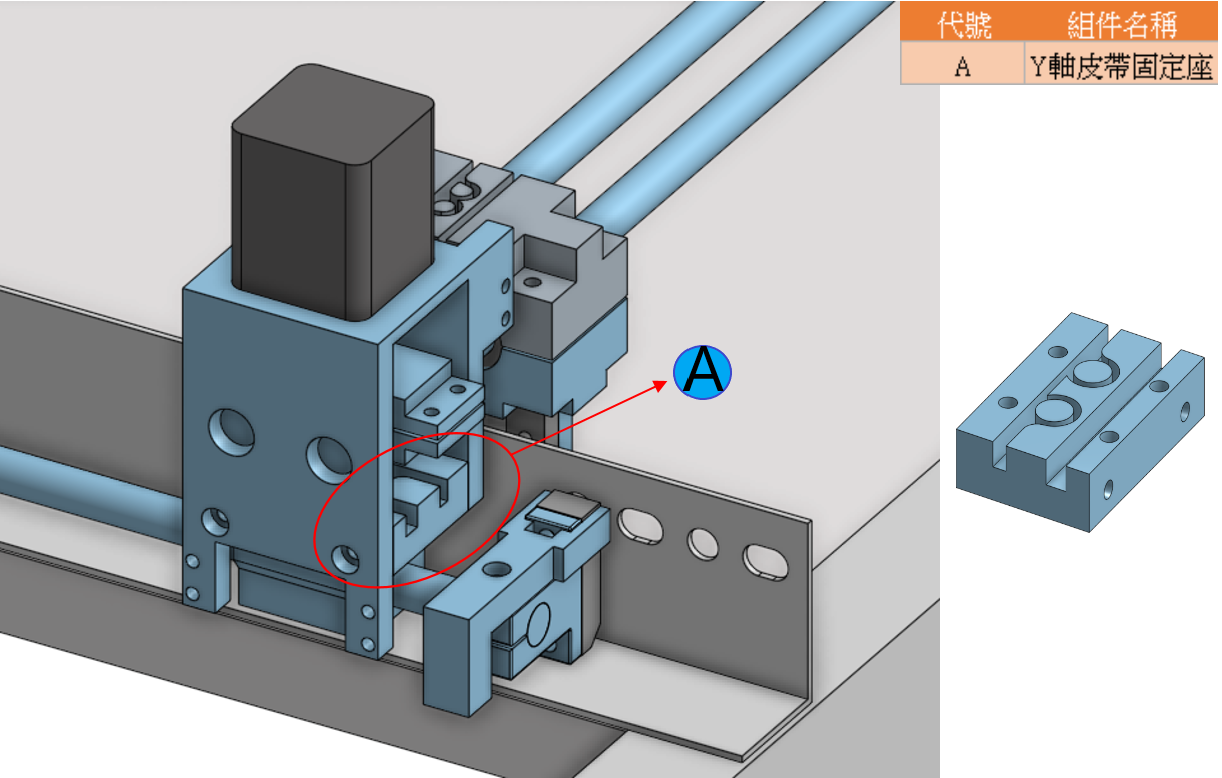
\includegraphics[width=8cm]{axialseat}
\caption{\Large Y軸皮帶固定座}
\label{axialseat}
\end{figure}

\begin{figure}[hbt!]
\center
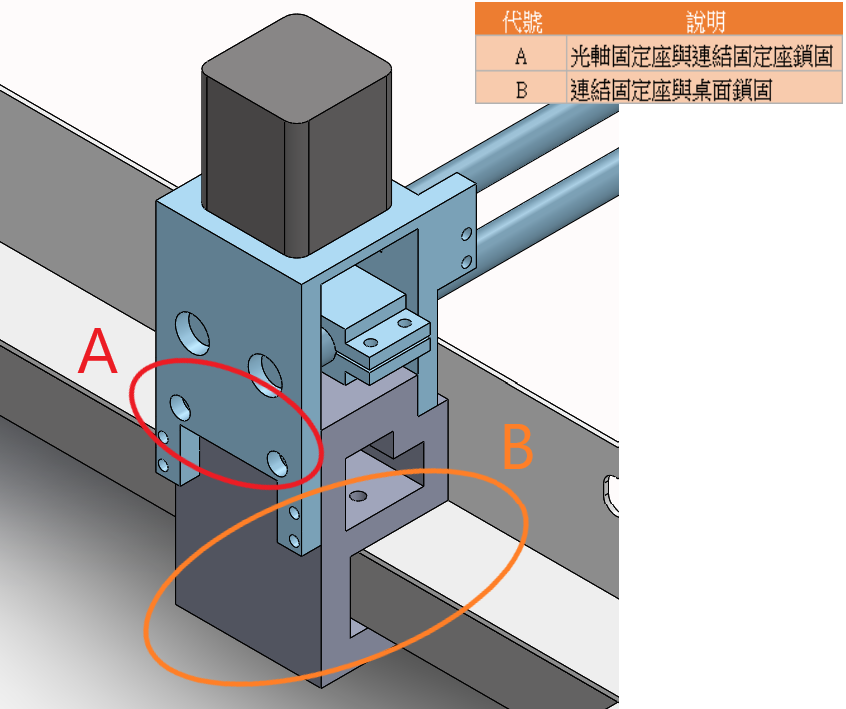
\includegraphics[width=8cm]{connectSeat}
\caption{\Large 連結固定座}
\label{connectSeat}
\end{figure}

\newpage
\qquad 分別在擊球器外側保留約冰球直徑1.5倍之區域作為得分判定區,如圖4.4中的紅色區域。\\
\section{CoppeliaSim模擬}
 CoppeliaSim是具有集成開發環境的機器人模擬器,基於分佈式控制體系架構,可以通過嵌入式腳本,插件,ROS或BlueZero節點,RemoteAPI客戶端或自定義解決方案進行模型控制。\\
 \begin{figure}[hbt!]
\center

\includegraphics[width=11cm]{CoppeliaSim}
\caption{\Large CoppeliaSim Logo}
\end{figure}

且CoppeliaSim中,控制器可以用C / C ++、Python、Java、Lua、Matlab或Octave編寫。\\
\subsection{使用原因}
 本專題之最終目標是希望可以在虛擬環境中進行深度強化學習來訓練機器對打,通過虛擬環境中的模擬後,可以更直接地看到深度強化學習訓練的狀況,且因為在虛擬環境中不會有金費的支出,所以可以不斷的重複模擬直到模擬達到最佳的狀態,除此之外CoppeliaSim的虛擬環境更接近真實環境,基於以上原因,所以使用了CoppeliaSim開發。\\
\subsection{RemoteAPI}
 RemoteAPI(Remote Application Programming Interface)是CoppeliaSim API框架的一部分。它允許CoppeliaSim與外部應用程序之間的通訊,是跨平台並支持服務調用和雙向數據流。有兩個不同的版本/框架分別為:Remote API 和The B0-based remote API。\\
\subsection{常用功能}
\begin{enumerate}
\item 以下為簡易功能說明:
\begin{figure}[hbt!]
\center
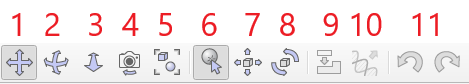
\includegraphics[width=11cm]{toolBar}
\caption{\Large CoppeliaSim 工具列}
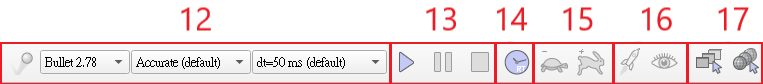
\includegraphics[width=13cm]{toolBar2}
\caption{\Large CoppeliaSim 工具列(續)}
\end{figure}
\begin{table}[hbt!]
\center
\large
\setlength{\tabcolsep}{0.75cm}{
\begin{tabular}{|c|c|c|c|}
\hline  代號 & 功能說明 & 代號 & 功能說明\\
\hline  1 &畫面平移& 10 &複製所有設定\\
\hline  2 &畫面旋轉& 11 &回復/取消回復\\
\hline  3 &畫面縮放&12&模擬設定\\
\hline  4 &畫面視角&13&開始/暫停/停止 模擬\\
\hline  5 &畫面縮放至適當大小&14&即時模擬切換\\
\hline  6 &選取物件&15&模擬速度控制\\
\hline  7 &移動物件&16&線程渲染/視覺化\\
\hline  8 &旋轉物件&17&場景/頁面 選擇\\
\hline  9 &加入/移出 樹狀結構&&\\
\hline 
\end{tabular}}
\caption{\Large 功能說明}
\end{table}
\newpage
%\item 模擬執行\\%
\end{enumerate}
\section{影像處理}

\qquad 在影像處理中我們主要使用了Python套件中的OpenCV(全稱:Open Source Computer Vision Library),並搭配其他套件或模組進行了影像處裡,藉此來取得訓練神經網路訓練時所需的資訊。\\
\begin{figure}[hbt!]
\center

\includegraphics[width=10cm]{pythonCVlogo}
\caption{\Large OpenCV 及Python logo}
\end{figure}

\subsection{CoppeliaSim中的Vision sensor(視覺傳感器)}
 CoppeliaSim的視覺傳感器輸出的影像是以每個像素中以RGB三個位元組所組成的,舉例來說:在CoppeliaSim中視覺傳感器取出畫面像素為512*256,則我們會接收到(512*256)像素*3=393,216個資料,是一筆相當大的資料,所以在影像處理上會消耗掉大量的資源。\\

\subsection{影像辨識}
 透過CoppeliaSim中的Vision sensor接收場景影像並輸出後,便可以開始進行影像辨識的處理。\\
\begin{enumerate}
\item RGB與HSV的轉換[\ref{RGBtoHSV}]\\
RGB即光的三原色Red(紅)Green(綠)Blue(藍),HSV則是一種將RGB色彩模型中的點在圓柱坐標系中的表示法,HSV分別表示Hue(色相)、Saturation(飽和度)、Value(明度),而會將RGB轉換為HSV是因為HSV相較於RGB可以更直接的判斷色彩、明暗和鮮豔度對於顏色過濾可以更方便定義出色彩範圍。\\
\begin{figure}[hbt!]
\center
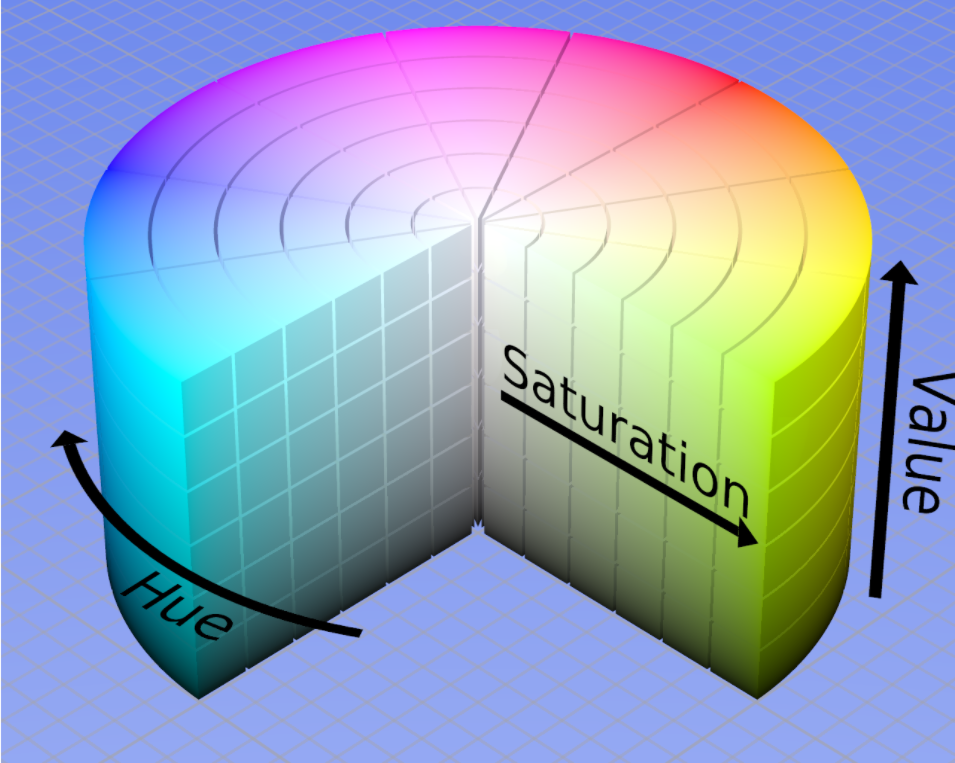
\includegraphics[width=10cm]{HSV}
\caption{\Large HSV色彩空間}
\end{figure}
\newpage
下列為RGB與HSV之間轉換的公式,首先是RGB轉為HSV,其中$max$及$min$分別為$(r,g,b)$中的最大與最小值:
$$h=\left\{\begin{matrix}
0^{\circ}, & \textrm{if}\ max=min\\ 
60^{\circ}+\frac{g-b}{max-min}+0^{\circ},& \textrm{if}\ max=r\;and\;g\geq \;b\\ 
60^{\circ}+\frac{g-b}{max-min}+360^{\circ}, & \textrm{if}\ max=r\;and\;g<  \;b\\ 
60^{\circ}+\frac{g-b}{max-min}+120^{\circ}, & \textrm{if}\ max=g\\ 
60^{\circ}+\frac{g-b}{max-min}+240^{\circ}, & \textrm{if}\ max=b
\end{matrix}\right.$$

$$s=\left\{\begin{matrix}
0, & \textrm{if}\,max=0\\ 
\frac{max-min}{max}=1-\frac{min}{max}, & \textrm{otherwise}
\end{matrix}\right.$$

$$v=max$$
接著是HSV轉為RGB:
$$\textrm{when}\,0\leq H< 360,0\leq S\leq 1,0\leq V\leq 1$$
$$C=V\times S$$
$$X=C\times (1-\left | (H/60^{\circ})\textrm{mod}2-1 \right |)$$
$$m=V-C$$

$$({R}',{G}',{B}')=\left\{\begin{matrix}
(C,X,0)& ,0^{\circ}\leq H< 60^{\circ}\\ 
 (X,C,0)& ,60^{\circ}\leq H< 120^{\circ}\\ 
 (0,C,X)& ,120^{\circ}\leq H< 180^{\circ}\\ 
 (0,X,C)& ,180^{\circ}\leq H< 240^{\circ}\\ 
 (X,0,C)& ,240^{\circ}\leq H< 300^{\circ}\\ 
 (C,0,X)& ,300^{\circ}\leq H< 360^{\circ}
\end{matrix}\right.$$


$$(R,G,B)=(({R}'+m)\times 255,({G}'+m)\times 255,({B}'+m)\times 255)$$

\item 顏色過濾\\
進行顏色過濾時,需要先定義出過濾顏色的上下限,在開始過濾後僅會保留介於上下界線範圍的影像,而介於上下限範圍之外的影像則會被剃除,如圖.\ref{filter}所示以上限(77,255,255)及下限(35,43,46)為例。\\
\begin{figure}[hbt!]
\center
\begin{minipage}[t]{0.48\textwidth}
\center
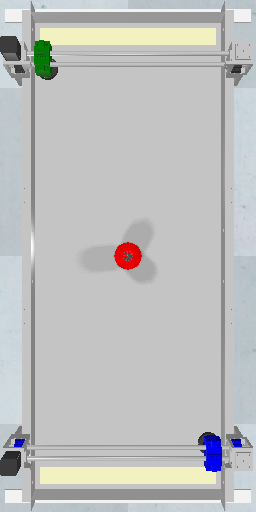
\includegraphics[width=6cm]{origin}
\caption{\Large 場景原圖}
\label{origin}
\end{minipage}
\begin{minipage}[t]{0.48\textwidth}
\center
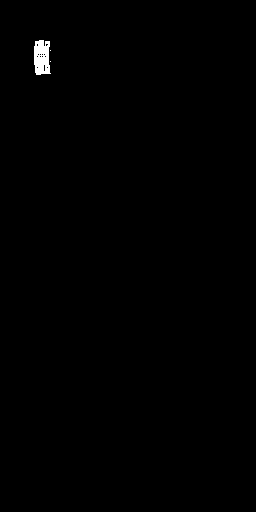
\includegraphics[width=6cm]{filter}
\caption{\Large 顏色過濾後的場景}
\label{filter}
\end{minipage}
\end{figure}


%\item 雜訊去除\\
%為了避免環境因素干擾,使影像產生雜訊並影響了影像辨識度,所以在雜訊的去除也是很重要的,

\end{enumerate}

\newpage
\chapter{伺服器}
 此專題採用 Ubuntu 20.04 版本作為我們的架設所使用作業系統,由於 Ubuntu 功能尤為繁多,以下說明重點只著重在專題製作所用到功能上。\\
 
 Ubuntu 作業系統是 Linux 系統的一個發行版,目前免費且開源,Ubuntu 基於 Debian發行版和 GNOME 桌面環境,其目標在於為一般使用者提供一個最新、穩定又主要以自由軟體建構而成的作業系統。\\
 
 其開發目的是為了使個人電腦變得簡單易用,它與其他基於 Debian 所發行的 Linux 版本更加接近 Debian 的開發理念,它主要使用自由、開源的軟體,而其他則帶很多閉源的軟體。\\
\section{Ubuntu 環境配置}
 在一開始會先使用套件管理系統 apt 指令去下載 Xorg , fluxbox , lxde 套件。Xorg 是 Ubuntu 操作系統的一個顯示服務器軟件包,它在被導入 Ubuntu 操作系統後會載入一系列的文件或軟件,這些都是跟顯示卡驅動,圖形環境庫相關的一些文件、軟件。Gnome ,kde,包括我們使用的 lxde 也需要 xorg 才能實現。而 Lxde 它的全名是 Lightweight X11 Desktop Environment ,是自由軟體桌面環境,其優點在於提供了輕量而快速的桌面環境,它比較重視實用、輕巧,除此之外它還可以在 Linux 平台執行。\\
 
 之後需選擇 display manager ( 顯示管理器 )的種類 ,Display manager 是操作系統 Ubuntu 的組件,其中登錄的動作即為 Display manager 負責。該操作系統中常見的類型有 gdm ,gdm3 , lightdm ,kdm ...。各類型的 Display manager 功能其實大同小異,差別在於外觀、操作、格式、複雜度和使用者感受等,可依使用者需求變更 ( 有些較為輕量,適合比較低階的運行器 )。選擇其中一個後繼續,之後可以切換更動 。\\

 再來是模組的導入,此處同樣用 apt 指令安裝:Pip , uwsgi , Nginx  , 以及 Git 。如果要從 Ubuntu 系統上安裝軟體,其中一種方式是 " pip "。「pip 」是 " pip Installs Packages " 的縮寫,是一個用命令列作為基礎的套件管理系統,可以用它來安裝 python 的應用程式。而使用 Git 是因為在備份資料時, 可幫助使用者有效管理原始碼,而 github 就是由 Git 伺服器和網頁介面組成,用來當作放置原始碼的倉庫。\\
 
 另外 Nginx 和 uwsgi 是為拿來配合把 python 程式應用在網路上實現,並且把想要的結果使其能在網路實時觀看操控結果之反饋。\\
\section{Oracle VM VirtualBox 介紹}
 假使建構虛擬環境時需要在同一主機使用不同電腦作業系統環境,則可使用「虛擬機器工作站」— Oracle VM VirtualBox 。\\

 選擇 Oracle VM VirtualBox    是為了因應當要使用不同作業系統 ( 比如本機與虛擬環境不同作業系統  ) 且不想與其資料存放時共用一個硬碟 ( 無多餘硬碟 , 不想硬碟之間有資料重疊 ... ) 時,即可使用其軟體做練習,降低操作失誤帶來的成本,而此軟體目前為免費,並隨時會更新,另外其特色有 :\\  
\begin{itemize}


\item 只要自備作業系統 ( 光碟片 , ISO映像檔 ) ,即可在啟動 Oracle VM VirtualBox  後直接開啟要操作的執行檔 ( 作業系統 ),不必再把主機本身重新關機,當然開啟多個作業系統之間也有共通性,可直接從視窗A做網路、檔案分享、複製貼上等動作到視窗B。\\
\item 除了作業系統裡面的執行,還可在其中練習磁碟分割、格式化以及 BIOS 啟動等 ( 但是未支援USB啟動 ) 。\\
\item 空間的佔用上並不是真實佔用空間,而是依據使用者的操作而變化 ( 使用者用多少就是多少 )。相對的,使用者雖然一開始設定該虛擬電腦的記憶體大小與硬碟空間是實時依據操作者決定,但終究還是佔掉電腦效能,所以 VirtualBox 的效能還是依據電腦本身的硬體配備。為了配置網路,首先在:
\begin{enumerate}
\item File / Preferences / Network  位置,新增一個或右鍵點擊現有的網路設定,填入該電腦網路設定 。
\item Settings / Network / Adapter 1 / Attached to: 該位置改成  Bridged Adapter
\end{enumerate}
\qquad 此處配置之比較 ( 取常用例子 ):NAT , Bridged , Internal , Host-only
\item NAT:最為基本之設定,主要讓該虛擬主機可連上網,但在與其他網路使用者互動時找不到該虛擬主機網路位址,外部網路也無法偵測,虛擬主機所有的網路請求都會把該來源視為宿主機的。
\item Host-only:虛擬主機被分配到一個網址,但是還是只有虛擬主機運行的環境可訪問該網路位址
\item Internal:此種設定主要為虛擬主機彼此間的連線,它可向外部提供資料,但反之則不行。
\item Bridged:在與其宿主機的網卡設定橋接與設定好外部網路位址後,可被外部網路訪問。
\end{itemize}
\newpage
\section{Web server}
 Nginx 是提供 web 相關服務的伺服器 ( Web server ),除了是高效能的 HTTP ( HTTPS ) 服務器外,還可處理靜態資源 , 負載平衡 , 代理等工作。代理工作為根據不同域名轉發到 Application Server 的不同 port 上去處理 ,其中又分正向和反向,正向代理為 clinet 端發送 request 經由 porxy server 再到目標網站,反向則反之。正向代理操作中 server 只知道 proxy server  給他 request , 不知道 client 是誰,而相同地反向代理則是 client 只知道 proxy server 給他 responses , 不知道 server 是誰。正向代理隐藏真實 Client,反向代理隱藏真實 Server。另外在高流量的狀況下,需要多個 Application Server 來分擔流量,負載平衡就是負責 request 的分發,決定 request 要被分到哪一個 Application Server 處理 。而關於處理靜態資源 ,Nginx 與 Apache 等 Web Server 處理靜態資源的能力是遠遠高於 Application Server 的。\\
\begin{figure}[hbt!]
\begin{center}
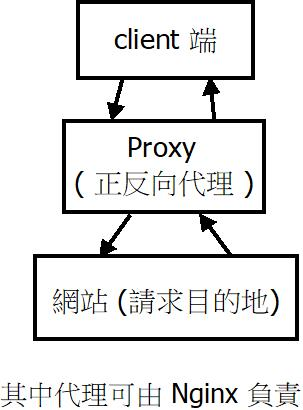
\includegraphics[scale=0.74]{clientProxy}
\caption{\Large clientProxy}\label{clientProxy}
\end{center}
\end{figure}

\section{Nginx}
\hspace{-1.7em} 網路設定:\\
 首先要修改網路設定檔,而其設定檔放在/etc/netplan目錄下的yaml檔。其中需更改的設定:
\begin{enumerate}
\item addresses:為靜態 IP,可以是IPV4或IPV6。
\item gateway:即為該電腦之閘道器。
\item nameservers:該電腦之DNS服務器。
\end{enumerate}

 WSGI(Python Web Server GateWay Interface)為一種用在Python語言上的規範,用來規範Web Server與Web Application之間如何溝通。而uWSGI同為實現了WSGI、uwsgi、http協議等的Web server,通常用於接收前端伺服器轉發的動態請求並轉發給Web Application。前者可以使用Nginx提供的https協定,且同上表述中Nginx的靜態資源處理能力較佳所以也能將靜態資源轉給其處理。\\
 
Nginx的主要設定檔nginx.conf可藉由include指令添加其他nginx設定檔的設定去擴增不同域名的設定,常見的設定有 :
\begin{enumerate}
\item 預設:
\begin{lstlisting}[caption=\Large nginx預設]
  reciveAPP {
    server localhost:5000;
    server localhost:5001;
}

server {
    listen 80;
    listen [::]:80;
    server_name SERVER_IP;
    root /home/hostname;

    location / {
            uwsgi_pass http://api/;
            include uwsgi_params;
    }
\end{lstlisting}

\newpage
\item 負載平衡LoadBalance:
\begin{lstlisting}[caption=\Large load balance設定]
  reciveAPP {
        ip_hash;
        server localhost:5000;
        server localhost:5001;
}

server {
    listen 80;
    listen [::]:80;
    server_name SERVER_IP;
    root /home/ryan;

    location / {
            uwsgi_pass 127.0.0.1:8000;
            include uwsgi_params;
    }
}
\end{lstlisting}
\end{enumerate}

 reciveAPP定義了將request proxy過去的應用,例子中server localhost語法代表可以請求proxy到分別監聽5000與5001 port的兩個應用,同時這個block可達到load balancer負載平衡的功能。\\
 
 server這個block則是定義了proxy server的相關設定,包括要監聽的port(listen 80為監聽所有IPV4位址,listen [::]80則為監聽所有IPV6位址)、規定哪些domain或ip的request會被 nginx server 處理(server\_ name)。\\
 
 location像是路由(routing)的概念,設定不同的path要對應到怎麼樣的設定。location中則是指對不同路徑的處理。\\
 
\begin{enumerate}
\item location:
\begin{lstlisting}[caption=\Large location設定]
  location / #匹配所有目錄

  location /static #匹配所有 /static 的開頭目錄
\end{lstlisting}
\end{enumerate}

 要達到load balancer透過一開始介紹的upstream block就可以達成,在上面的例子中,來自某個domain 80 port會被分配到port 5000或port 5001兩個應用中,達成用兩個應用去分擔request的負載平衡器。\\
 
 負載平衡裡的負載規則(ip\_hash )某個request要被導倒哪個應用去處理有不同規則,每個規則都有各自適合使用時機,以下簡單介紹幾個常見的規則:\\

\begin{enumerate}
\item round-robin(預設)輪詢方式:也就是將請求輪流按照順序分配給每一個 server。假設所有伺服器的處理效能都相同,不關心每臺伺服器的當前連線數和響應速度。適合於伺服器組中的所有伺服器都有相同的軟硬體配置並且平均伺服器請求相對均衡的情況。
不過也有另外一種可以設定權重的Weight Round Robin(加權輪詢方式),可以設定不同server的權重,例如以下範例:
\begin{lstlisting}[caption=\Large 設定不同 server 的權重]
  upstream myweb {
    server web1.dtask.idv.tw weight=3;
    server web2.dtask.idv.tw weight=2;
}
\end{lstlisting}
\item least-connected 最少連線:顧名思義為連線進來時會把Request導向連線數較少的Server。
\item IP-hash依據Client IP來分配到不同台Server:通過一個雜湊(Hash)函式將一個 IP 地址對映到一臺伺服器。先根據請求的目標IP地址,作為雜湊鍵(Hash Key)從靜態分配的散列表找出對應的伺服器。除非斷線或IP變動,否則同個IP的請求都會導入到同一個 server。
\end{enumerate}
  uWSGI設定(uwsgi\_ini ):
 \begin{enumerate} 
 \item wsgi-file:主要運行的py檔案
 \item http,socket,http-socket:端口設定,假使有使用到 前端服務器(如Nginx)時,不能用http設定,因uwsgi協議為HTTP,而Nginx使用傳輸協議為TCP,兩者不能互通。
 \begin{lstlisting}[caption=\Large 簡易uwsgi指令啟動]
  uwsgi --http:9000 --wsgi-file APP.py 
\end{lstlisting}
 \item processes、threads:工作序,processes為進程,threads為線程,下方設定為每條近程有兩條線程。
 \begin{lstlisting}[caption=\Large 加入工作程序uwsgi指令啟動]
  uwsgi --http:9000 --wsgi-file APP.py --processes 4 --threads 2
\end{lstlisting}
\item chdir:此項是為了正確的加載模組/檔案 \\
整體快速配置(這裡儲存成一個.ini文件,其他還有YAML、JSON、XML格式等):
\begin{lstlisting}[caption=\Large 將uwsgi指令啟動動作設定成一個啟動檔]
  [uwsgi]
socket = :9000
processes = 4
threads = 2
chdir = location/to
wsgi-file = location/to/file
\end{lstlisting}
此項還可加上status:此項為查看uWSGI內部的輸出數據\\
\begin{lstlisting}[caption=\Large status]
  -- status 127.0.0.1:9001
\end{lstlisting}
實現之通訊流程 

\begin{figure}[hbt!]
\begin{center}
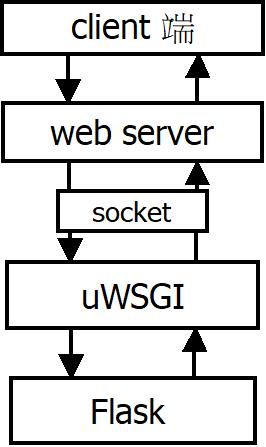
\includegraphics[scale=0.74]{clientToflask}
\caption{\Large client To flask}\label{clientToflask}
\end{center}
\end{figure}
 \end{enumerate}
\section{Flask}
 
 如同以上所述,建立Flask框架的同時需選擇反向代理伺服器(這裡我們選擇了Nginx)來負責網頁請求和結果的回覆,同時還需要一個實現WSGI通信協議的伺服器(我們選擇了 uWSGI)來負責接收代理伺服器的請求後Flask轉發及接收訊息,再轉發回去(代理伺服器)。\\
 
\begin{figure}[hbt!]
\begin{center}
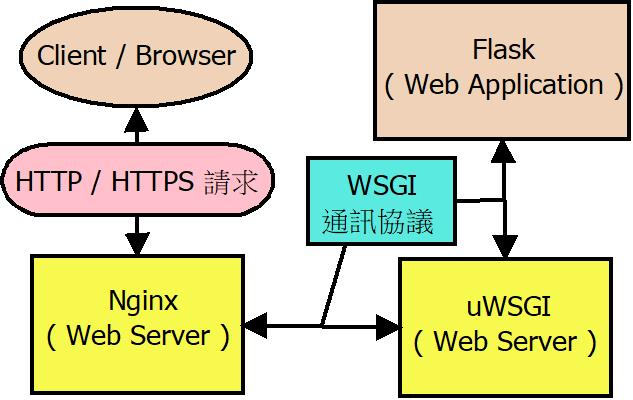
\includegraphics[scale=0.74]{total}
\caption{\Large total}\label{total}
\end{center}
\end{figure}

\chapter{機器學習的訓練與模擬控制結果}

\chapter{未來研究建議}
本專題已建立2D環境的算法與訓練數據,並將實體系統導入虛擬環境,建立跨平台控制(RemoteAPI)及輔助對打系統,後續可透過建立虛擬環境的訓練程式進行虛擬訓練,完成虛擬訓練後可導入實體機電系統,將對打系統實體化,架設伺服器提供網際介面,提供網際控制、即時觀看對打影像等功能。
\begin{figure}[hbt!]
\begin{center}
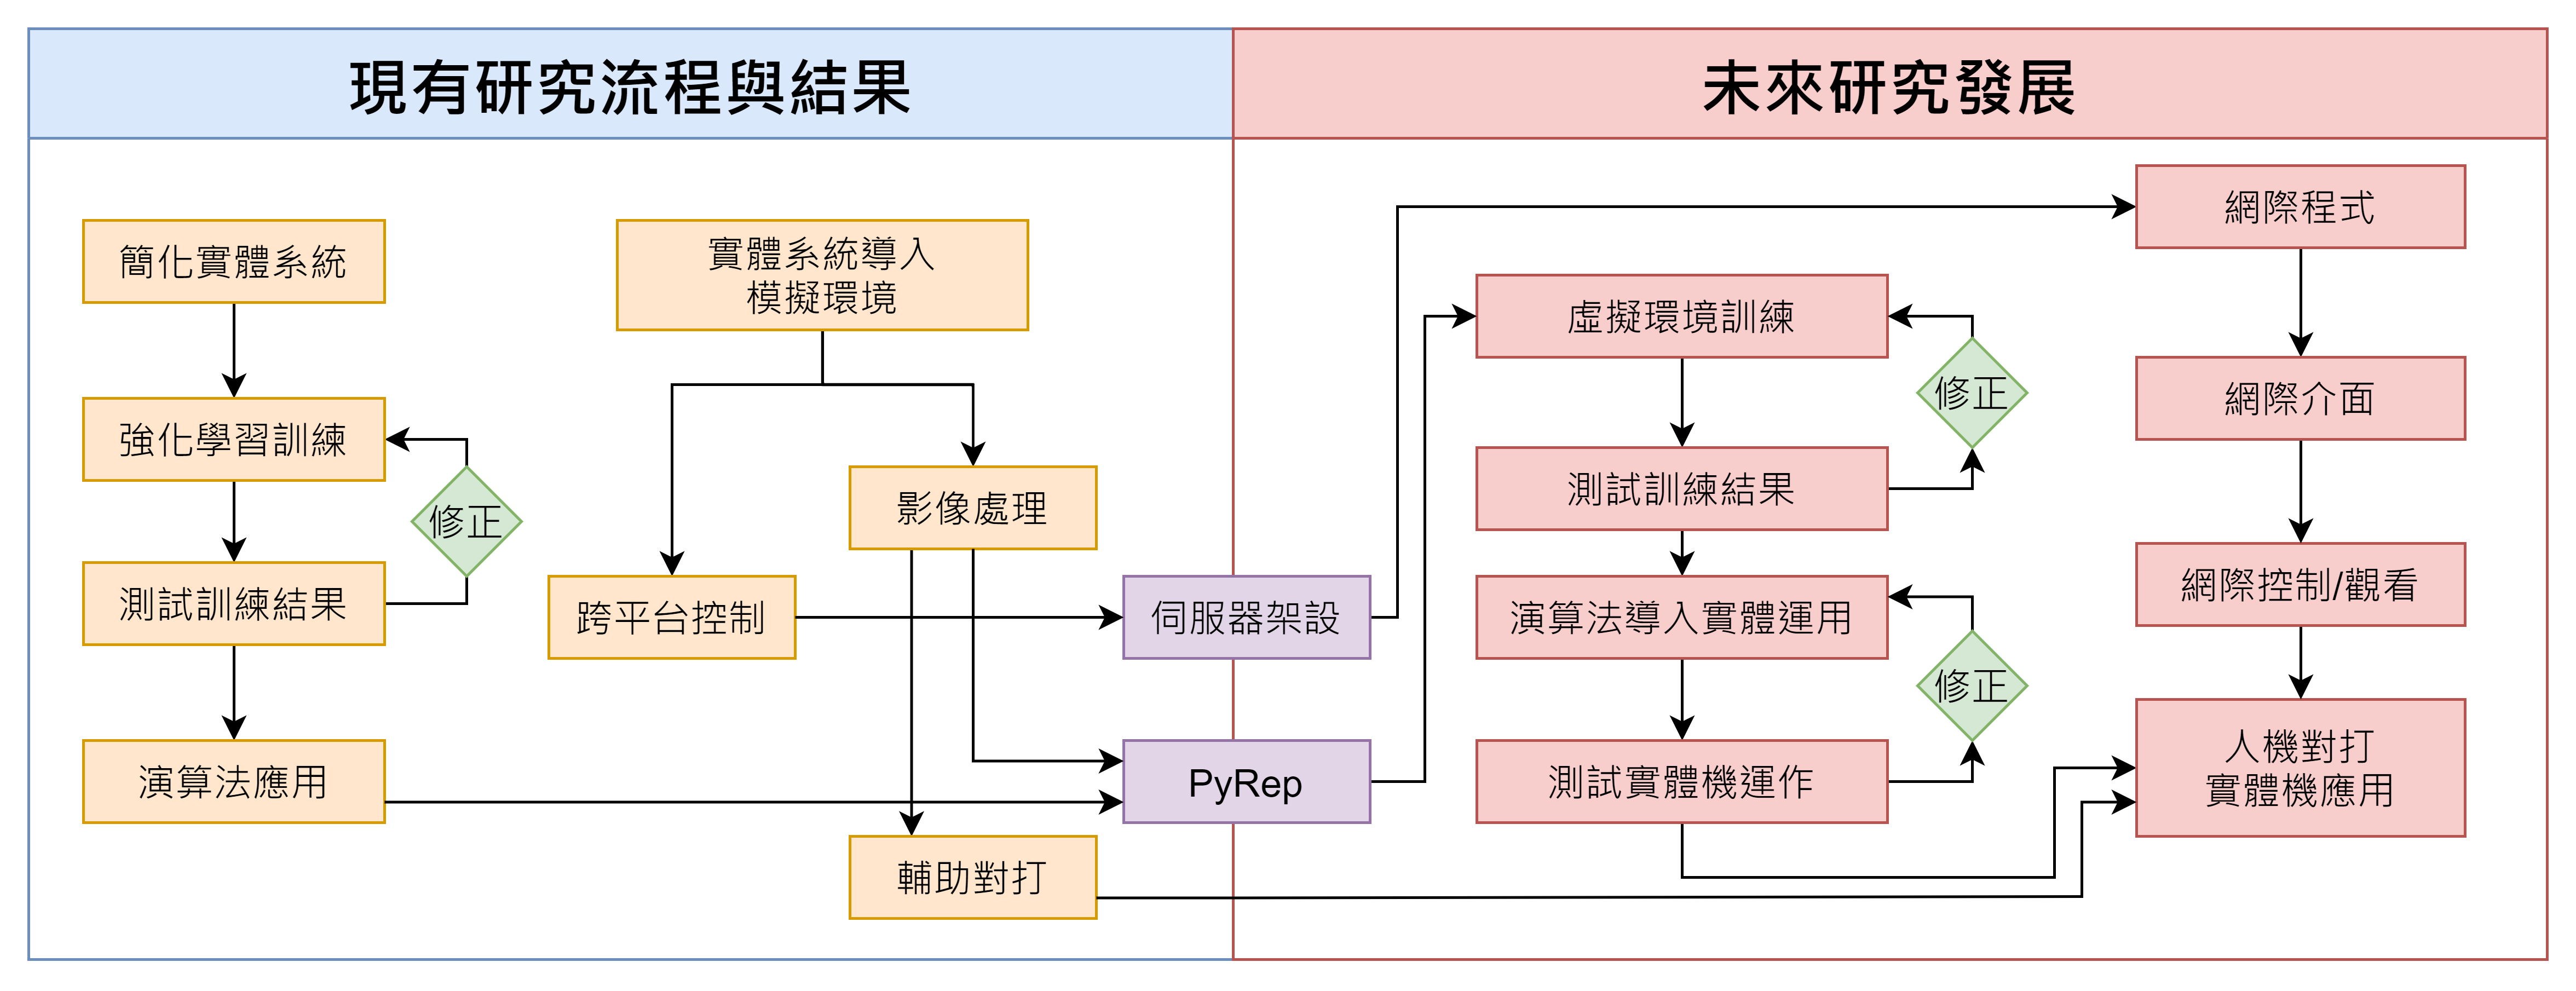
\includegraphics[width=16cm]{現有研究流程與未來展望}
\caption{\Large 現有研究流程與未來展望}
\label{fig.現有研究流程與未來展望}
\end{center}
\end{figure}

\chapter{問題與討論}
\hspace{-1.7em} Q:gym用到的atari動態連結庫在讀取目錄下但在執行的時候出現缺少 ale\_ c.cp38-win\_ amd64.dll\\
\begin{figure}[hbt!]
\begin{center}
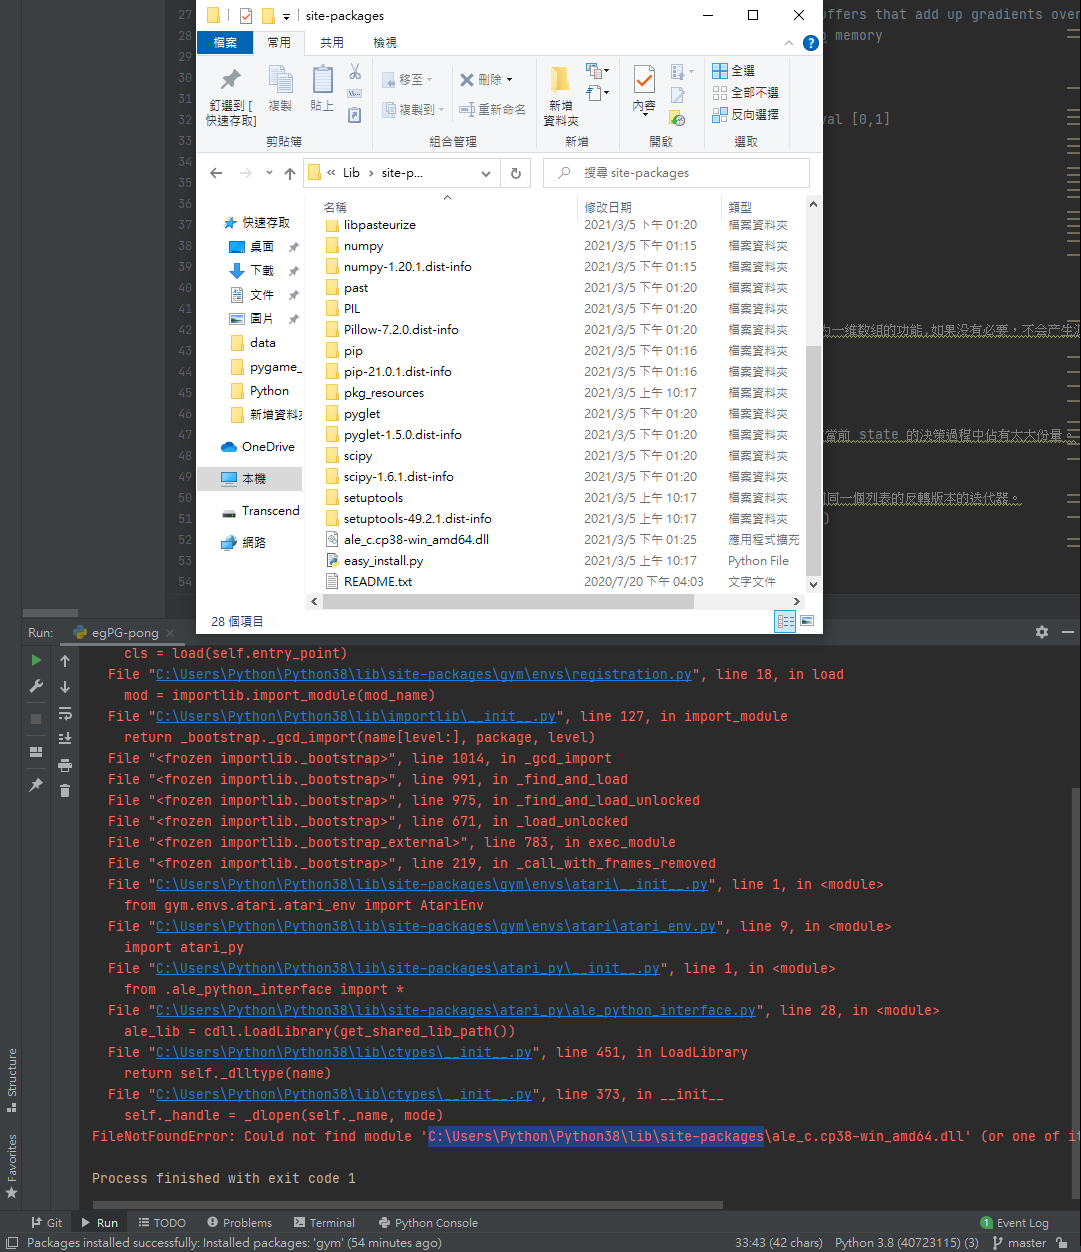
\includegraphics[width=15cm]{Q_dll}
\caption{\Large 動態連結庫錯誤}
\label{fig.動態連結庫錯誤}
\end{center}
\end{figure}
\newpage
\hspace{-1.4em}A:此問題尚未找到解決方法。\\
Q:錄製訓練過程的程式讀不到ffmpeg(圖.\ref{fig.Q_ffmpeg})。\\
\begin{figure}[hbt!]
\begin{center}
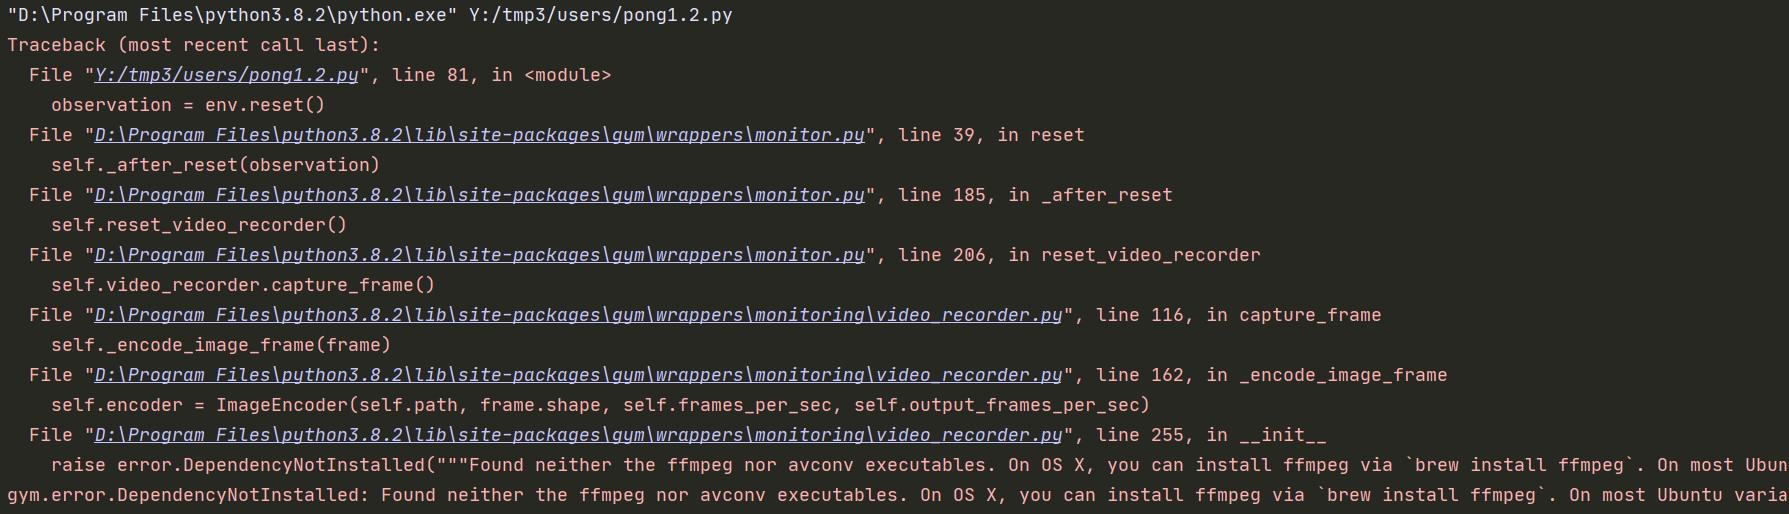
\includegraphics[width=15cm]{Q_ffmpeg}
\caption{\Large 程式讀不到ffmpeg}
\label{fig.Q_ffmpeg}
\end{center}
\end{figure}
\qquad \\
A:需要在作業系統中安裝ffmpeg:
\begin{enumerate}
\item 下載、解壓縮\\
先到官網 \href{https://ffmpeg.org/download.html}{https://ffmpeg.org/download.html} 下載" \href{https://www.gyan.dev/ffmpeg/builds/}{Windows builds from gyan.dev} ",下載 \href{https://www.gyan.dev/ffmpeg/builds/ffmpeg-git-full.7z}{https://www.gyan.dev/ffmpeg/builds/ffmpeg-git-full.7z} ,解壓縮重新命名成"ffmpeg"並放到C槽目錄下(C:$\setminus$ffmpeg)。
\item 環境設定(windows10 20H2 及 2004版本)\\
開啟"設定"→"系統"→左方"關於"選項→右側"進階系統設定"→"環境變數"(圖.\ref{fig.Q_ffmpeg-2})→選取"Path",編輯(圖.\ref{fig.Q_ffmpeg-3})→"新增",增加一個環境變數,給定內容為:"C:$\setminus$ffmpeg$\setminus$bin","確定"(圖.\ref{fig.Q_ffmpeg-4})→"確定"→"確定\\
\end{enumerate}
\begin{figure}[hbt!]
\begin{center}
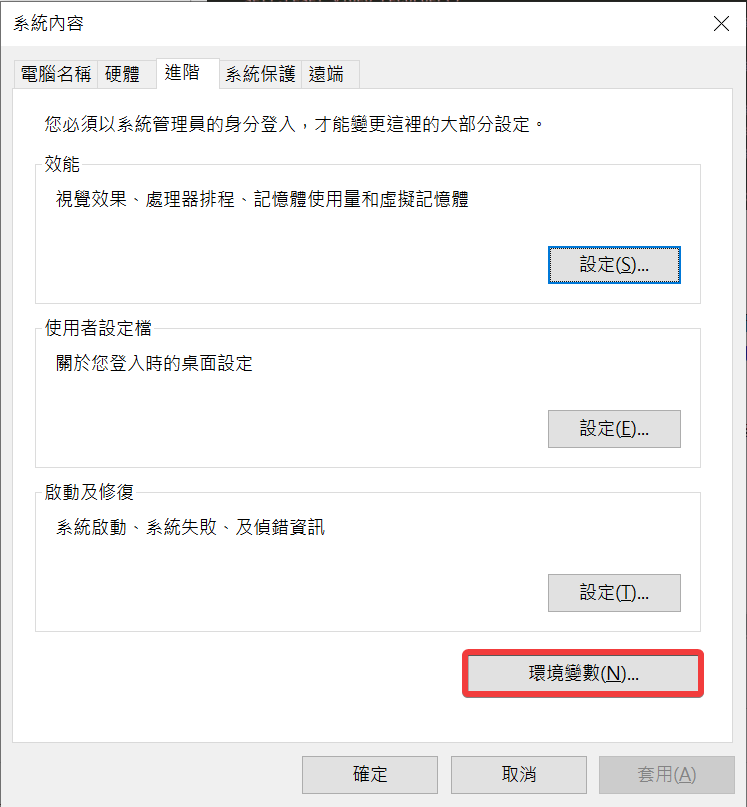
\includegraphics[width=10cm]{Q_ffmpeg-2}
\caption{\Large 進階系統設定}
\label{fig.Q_ffmpeg-2}
\end{center}
\end{figure}
\fontsize{0.001pt}{1pt}\selectfont .\\ %圖片間距勿刪
\begin{figure}[hbt!]
\begin{center}
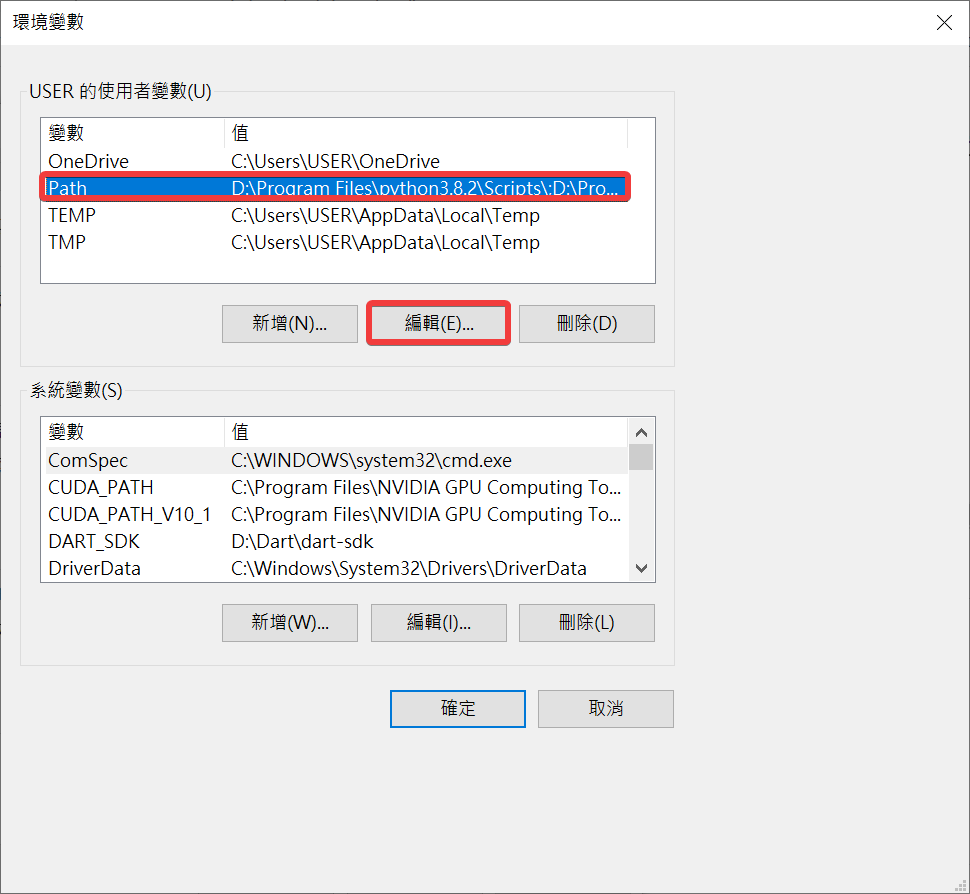
\includegraphics[width=10cm]{Q_ffmpeg-3}
\caption{\Large 環境變數}
\label{fig.Q_ffmpeg-3}
\end{center}
\end{figure}
\fontsize{0.001pt}{1pt}\selectfont .\\ %圖片間距勿刪
\newpage
\begin{figure}[hbt!]
\begin{center}
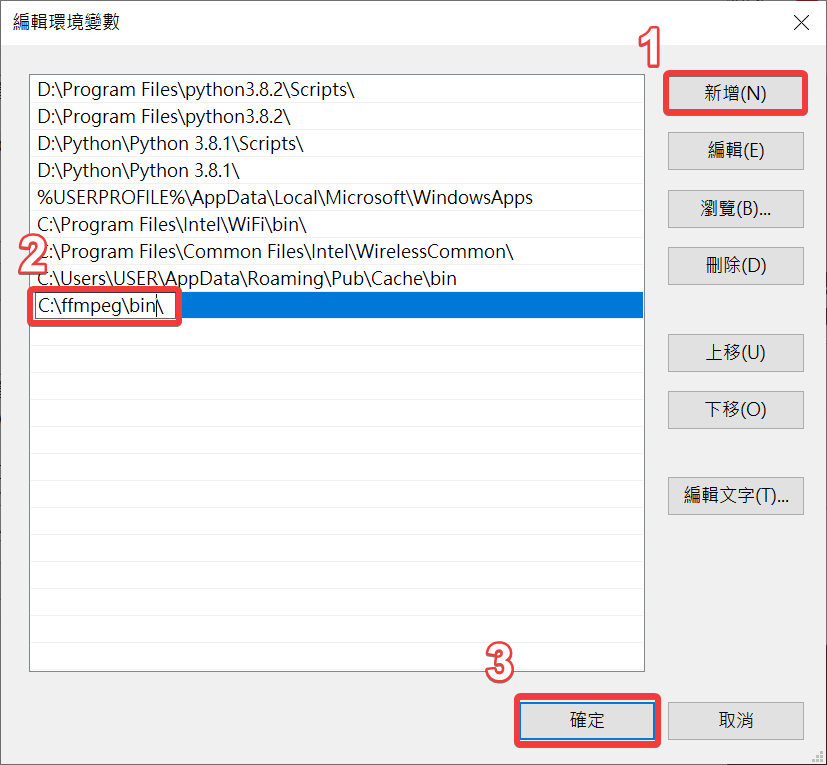
\includegraphics[width=15cm]{Q_ffmpeg-4}
\caption{\Large 編輯環境變數}
\label{fig.Q_ffmpeg-4}
\end{center}
\end{figure}
\fontsize{0.001pt}{1pt}\selectfont .\\ %圖片間距勿刪

\newpage %圖片間距勿刪
\fontsize{14pt}{28pt}\selectfont

\begin{itemize}
\item 測試\\
開啟命令字元(win+R,輸入"cmd"),執行"ffmpeg"(圖.\ref{fig.Q_ffmpeg-5})\\

\begin{figure}[hbt!]
\begin{center}
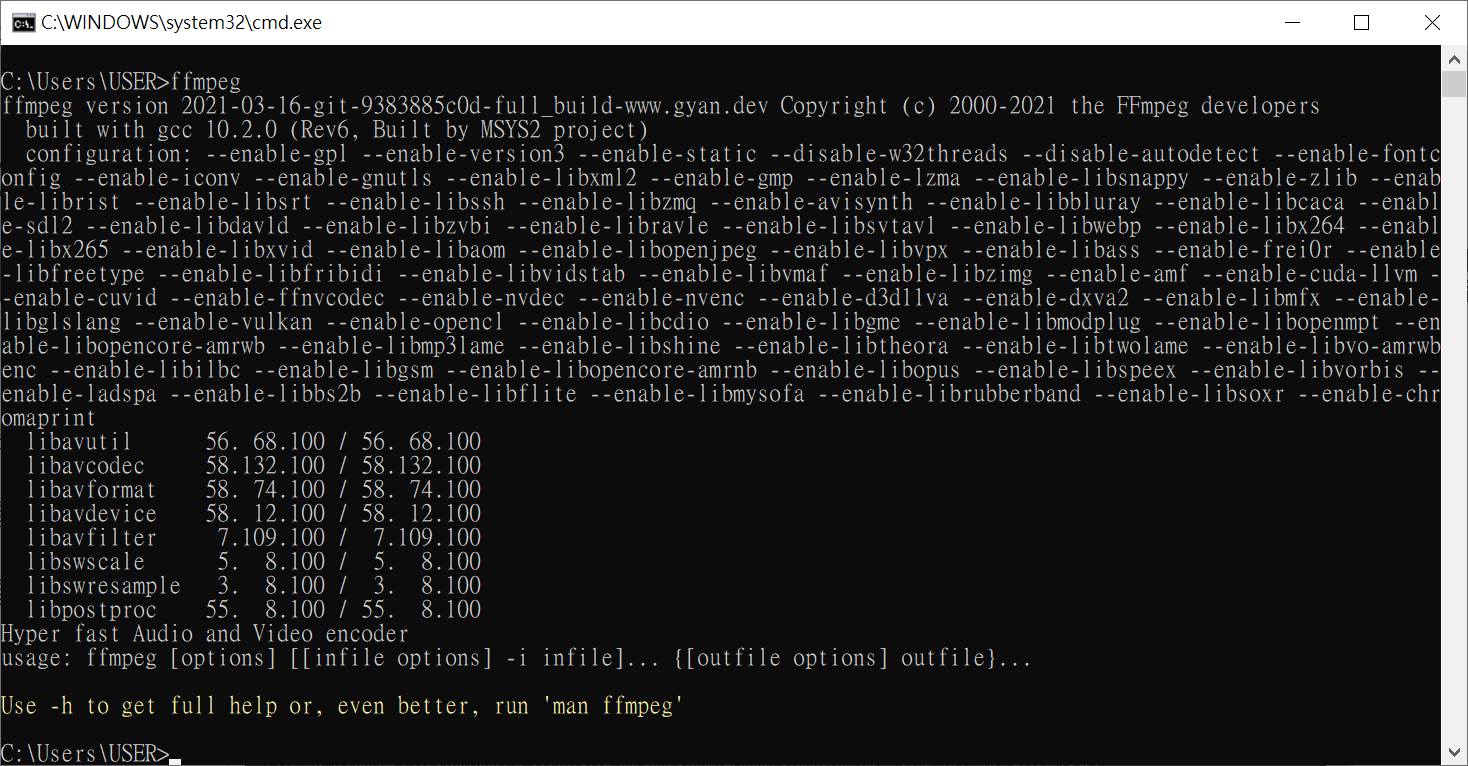
\includegraphics[width=15cm]{Q_ffmpeg-5}
\caption{\Large ffmpeg成功執行}
\label{fig.Q_ffmpeg-5}
\end{center}
\end{figure}
\end{itemize}
\newpage%圖片間距勿刪
\hspace{-1.7em} Q:運用gym.wrappers.Monitor透過ffmpeg進行錄影,紀錄下訓練影像。但記錄後的影像資料皆為1KB,並且無法開啟。(圖.\ref{fig.ffmpeg_mp4})\\
\begin{figure}[hbt!]
\begin{center}
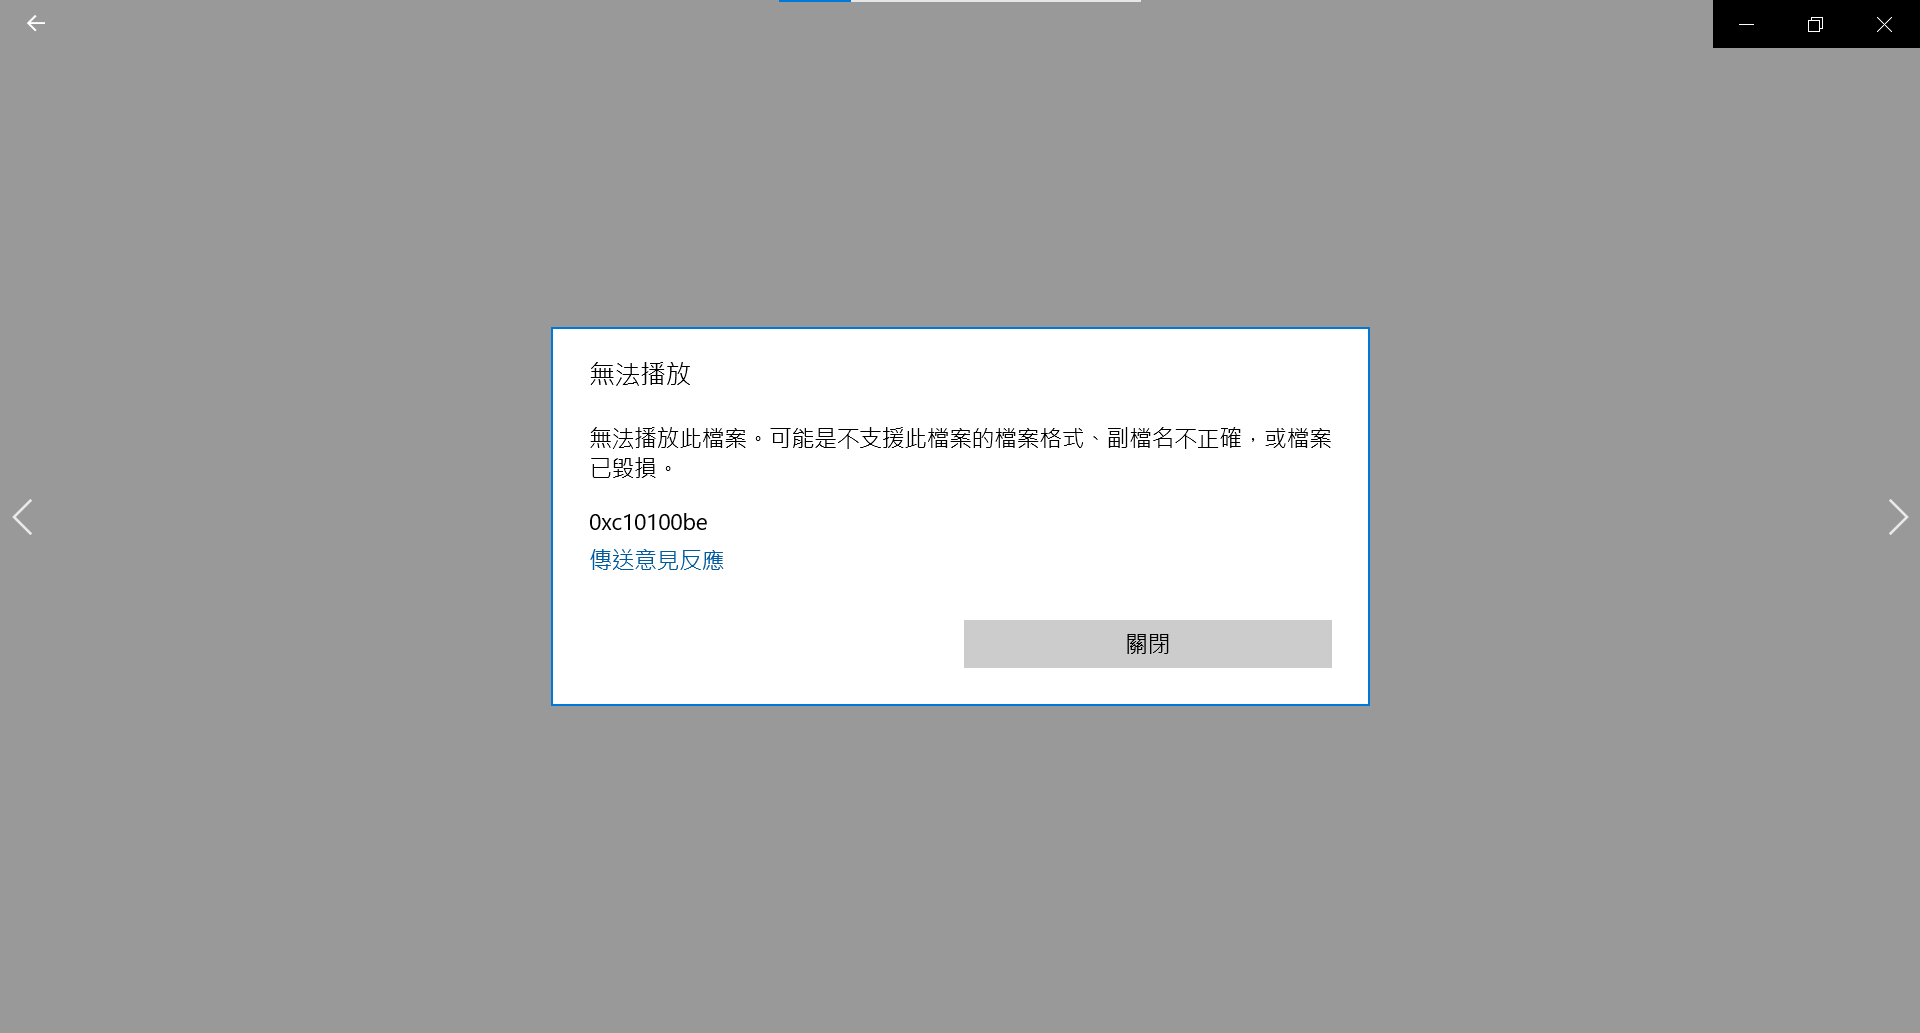
\includegraphics[width=15cm]{ffmpeg_mp4}
\caption{\Large 錄製後,影片無法開啟}
\label{fig.ffmpeg_mp4}
\end{center}
\end{figure}
\qquad \\%圖片間距勿刪
%圖片間距勿刪
A:修改g ym.wrappers.Monitor的video\_ recorder.py的設定(圖.\ref{fig.video_recorder}),將303行的縮排修正(從if階層上移到def的階層)即可(圖.)。\\
\begin{figure}[hbt!]
\begin{center}
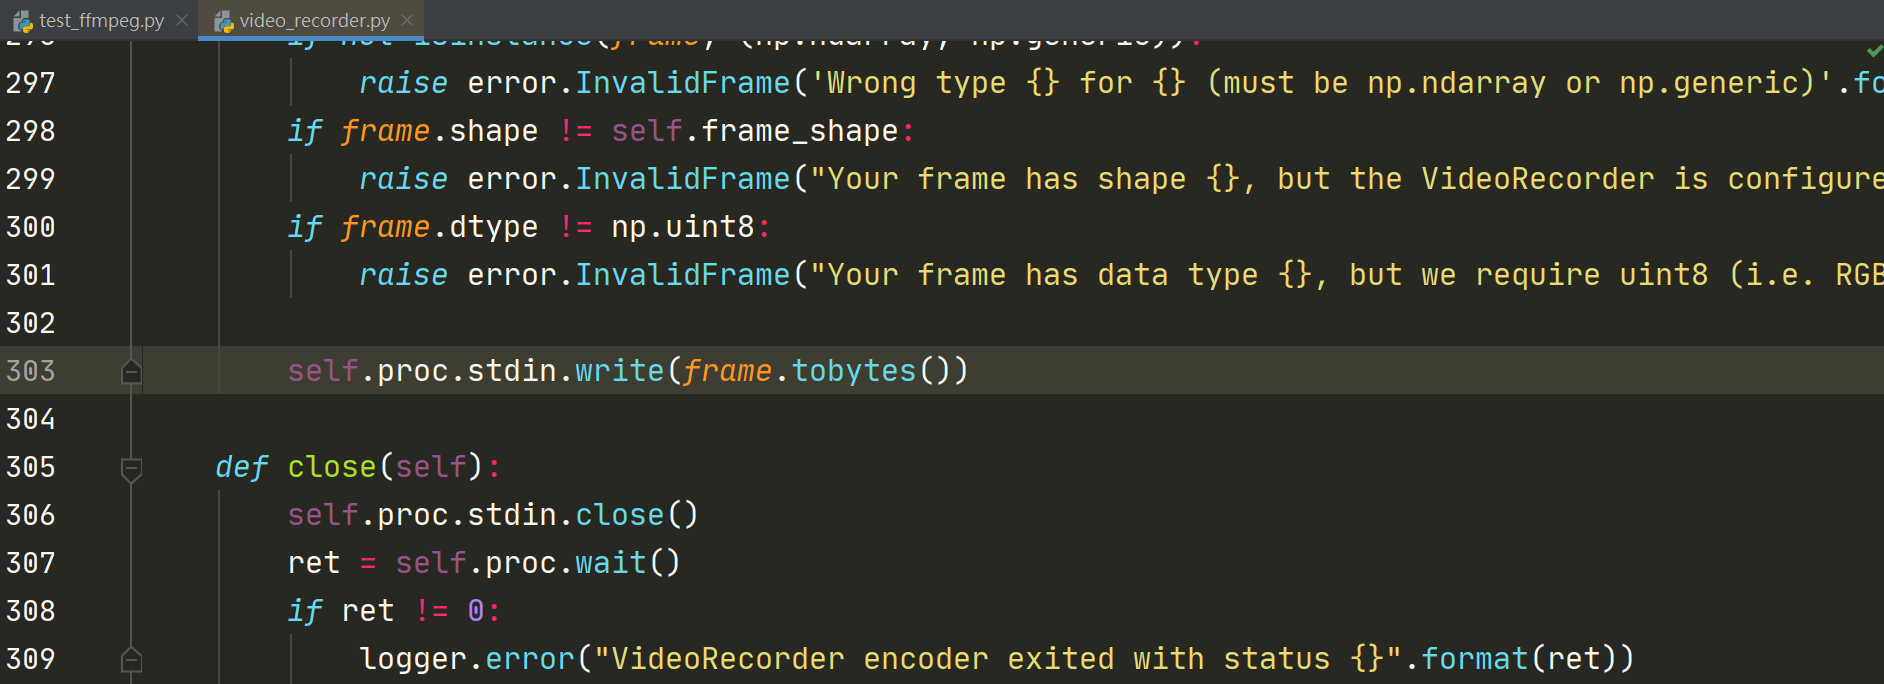
\includegraphics[width=15cm]{video_recorder}
\caption{\Large 原始設定}
\label{fig.video_recorder}
\end{center}
\end{figure}

\begin{figure}[hbt!]
\begin{center}
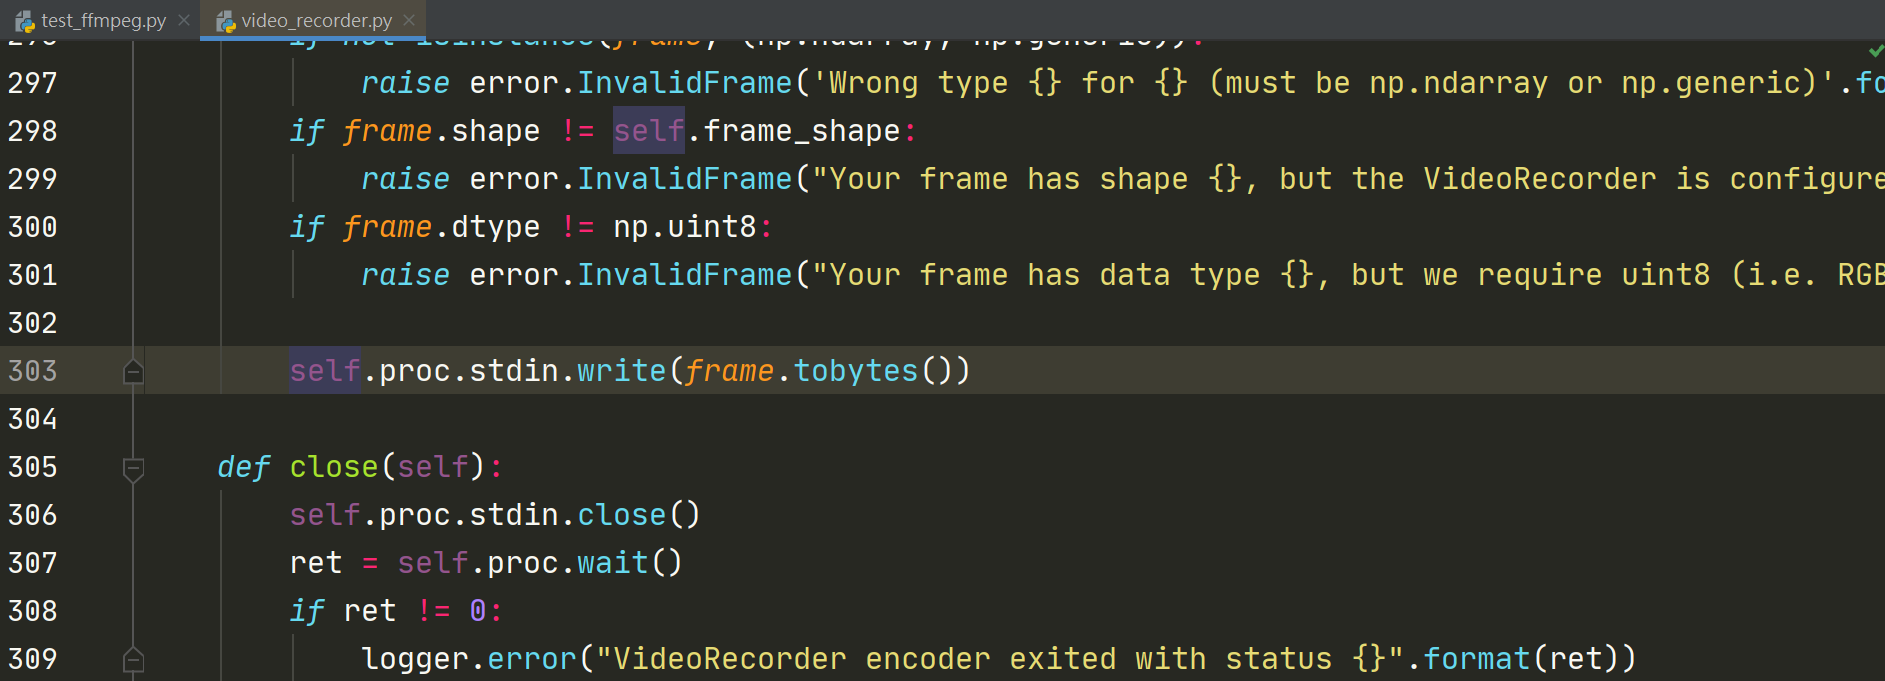
\includegraphics[width=15cm]{修正video_recorder}
\caption{\Large 修正後設定}
\label{fig.修正video_recorder}
\end{center}
\end{figure}
\newpage %圖片間距勿刪

\hspace{-1.7em} Q:啟用cmsimde的MathJax的功能遇到文章使用括號補充說明的內容被誤當成latex的語法轉換。\\
\hspace{-1.7em} A:格式轉換原始定義成"("和")",所以出現誤換的問題。\\
\begin{lstlisting}[caption=\Large\sectionef MathJax 程式碼]
<script>
  MathJax = {
    tex: {inlineMath: [['$', '$'], ['\\(', '\\)']]}
  };
  </script>
  <script id="MathJax-script" 
  async src="https://cdn.jsdelivr.net/npm/mathjax@3/es5/tex-chtml.js"> 
  </script>
\end{lstlisting}

修正後將"("和")"換成"\$",就解決誤換問題
%=---------------------參考文獻----------------------=%
\addcontentsline{toc}{chapter}{參考文獻} %新增目錄名稱
\newpage
\renewcommand\bibname{參~考~文~獻}
\begin{thebibliography}{99}  % 參考文獻印出之編號最寬為兩個字母寬
\bibitem 1\href{https://towardsdatascience.com/adam-latest-trends-in-deep-learning-optimization-6be9a291375c}{https://towardsdatascience.com/adam-latest-trends-in-deep-learning-optimization-6be9a291375c}
\bibitem 2\href{https://towardsdatascience.com/derivative-of-the-sigmoid-function-536880cf918e}{https://towardsdatascience.com/derivative-of-the-sigmoid-function-536880cf918e}
\bibitem 3\href{http://www.incompleteideas.net/book/RLbook2020.pdf}{http://www.incompleteideas.net/book/RLbook2020.pdf}
\bibitem 4\href{https://medium.com/change-the-world-with-technology/policy-gradient-181d43a24cf5}{https://medium.com/change-the-world-with-technology/policy-gradient-181d43a24cf5}
\bibitem 5\href{https://livebook.manning.com/book/grokking-deep-reinforcement-learning/chapter-11/v-11/38}{https://livebook.manning.com/book/grokking-deep-reinforcement-learning/chapter-11/v-11/38}
\bibitem 6\href{http://ukko.life.nctu.edu.tw/~u0517047/usage.html}{http://ukko.life.nctu.edu.tw/~u0517047/usage.html}
\bibitem 7\href{https://lilianweng.github.io/lil-log/2018/04/08/policy-gradient-algorithms.html}{https://lilianweng.github.io/lil-log/2018/04/08/policy-gradient-algorithms.html}\label{R.Policy Gradient}
\bibitem 8\href{https://uupgrade.medium.com/python-那些年我們一起玩過的遊戲-三-打磚塊-d89b648896ca}{https://uupgrade.medium.com/python-那些年我們一起玩過的遊戲-三-打磚塊-d89b648896ca}
\bibitem 9\href{https://cvfiasd.pixnet.net/blog/post/275774124-深度學習激勵函數介紹}{https://cvfiasd.pixnet.net/blog/post/275774124-深度學習激勵函數介紹}
\bibitem 0\href{https://www.coppeliarobotics.com/helpFiles/}{https://www.coppeliarobotics.com/helpFiles/}
\bibitem 1\href{https://hackernoon.com/the-reason-behind-moving-in-the-direction-opposite-to-the-gradient-f9566b95370b}{https://hackernoon.com/the-reason-behind-moving-in-the-direction-opposite-to-the-gradient-f9566b95370b}\label{OGD}
\bibitem 2\href{https://ruder.io/optimizing-gradient-descent/}{https://ruder.io/optimizing-gradient-descent/}
\label{OGD2}
\bibitem 3\href{https://reurl.cc/43XjEL}{https://zh.wikipedia.org/wiki/HSL和HSV色彩空間}
\label{RGBtoHSV}
\bibitem 4\href{https://reurl.cc/gzMm4N}{https://gist.github.com/karpathy/a4166c7fe253700972fcbc77e4ea32c5\# file-pg-pong-py}\label{R.pong1}
\bibitem 5\href{https://reurl.cc/95172Y}{https://github.com/schinger/pong\_ actor-critic/blob/master/pg-pong-ac.py}\label{R.pong1.1}
\bibitem 6\href{https://gist.github.com/etienne87/6803a65653975114e6c6f08bb25e1522}{https://gist.github.com/etienne87/6803a65653975114e6c6f08bb25e1522}\label{R.pong2}
%\bibitem 7\href
%\bibitem 8\href
%
%\bibitem 3\href{https://blog.csdn.net/Csdn_Darry/article/details/107142216}{https://blog.csdn.net/CsdnDarry/article/details/107142216}
\end{thebibliography}
\newpage
%=---------------附錄-----------------=%
\addcontentsline{toc}{chapter}{附錄} %新增目錄名稱
\begin{appendix}
\renewcommand{\thesection}{\bf 附錄 \Alph{section}}%設定標題名稱
\begin{center}
\fontsize{20pt}{0em}\selectfont\bf 附錄
\end{center}
\section*{LaTeX}
LaTex 為一種程式語言,支援標準庫 (Standard Libraries) 和外部程式庫 (External Libraries),不過與一般程式語言不同的是,它可以直接表述 Tex 排版結構,類似於 PHP 之於 HTML 的概念。但是直接撰寫 LaTex 仍較複雜,因此可以藉由 Markdown 這種輕量的標註式語言先行完成文章,再交由 LaTex 排版。
此專題報告採用編輯軟體為LaTeX,綜合對比Word編輯方法,LaTeX較為精準正確、更改、製作公式等,以便符合規範、製作。
 \begin{table}[htbp] %htbp代表表格浮動位置
			\centering%表格居中
			\caption{文字編輯軟體比較表}%表:標題
			\large%字體大小
			\label{tab_文字編輯軟體比較表:scale}
			\begin{tabular}{|c|c|c|c|c|c|c|}
			\hline
			\diagbox[width=5em]& 相容性 & 直觀性 & 文件排版 & 數學公式 & 微調細部\\ 
			\hline
			LaTeX 		&$\surd$&		&$\surd$&$\surd$&$\surd$\\
			\hline
			Word	 	&		&$\surd$&		&		&$\surd$\\
			\hline
			
			\end{tabular}
		\end{table}	

\begin{itemize} 
\item 特點:
\end{itemize}
\begin{enumerate}
\item 相容性:以Word為例會有版本差異,使用較高版本編輯的文件可能無法以較低的版本開啟,且不同作業系統也有些許差異;相比LaTeX可以利用不同編譯器進行編譯,且為免費軟體也可移植至可攜系統內,可以搭配Github協同編譯。
\item 文件排版:許多規範都會要求使用特定版型,使用文字編譯環境較能準確符合規定之版型,且能夠大範圍的自定義排定所需格式,並能不受之後更改而整體格式變形。
\item 數學公式呈現:LaTex可以直接利用本身多元的模組套件加入、編輯數學公式,在數學推導過程能夠快速的輸入自己需要的內容即可。
\item 細部調整:在大型論文、報告中有多項文字、圖片、表格,需要調整細部時,要在好幾頁中找尋,而LaTeX可以分段章節進行編譯,再進行合併處理大章節。
\end{enumerate}
\begin{figure}[hbt!]
\begin{center}
\includegraphics[width=10cm]{}
\caption{\Large 編譯流程}
\label{fig.編譯流程}
\end{center}
\end{figure}
\end{appendix}
\section*{FFmpeg}
FFmpeg是一個開放原始碼的自由軟體,可以對音訊和視訊進行多種格式的錄影、轉檔、串流功能。在專題訓練過程中透過FFmpeg的視訊錄製的功能記錄對打影像來了解實際訓練狀況。
\newpage

\newpage
%=-------------作者簡介-----------------=%
    \addcontentsline{toc}{chapter}{作者簡介}
    \begin{center}
	\fontsize{20pt}{0em}\selectfont \bf{作者簡介}\\
	\end{center}	
	{\begin{textblock}{6}(0,0.5)
	\begin{figure}
	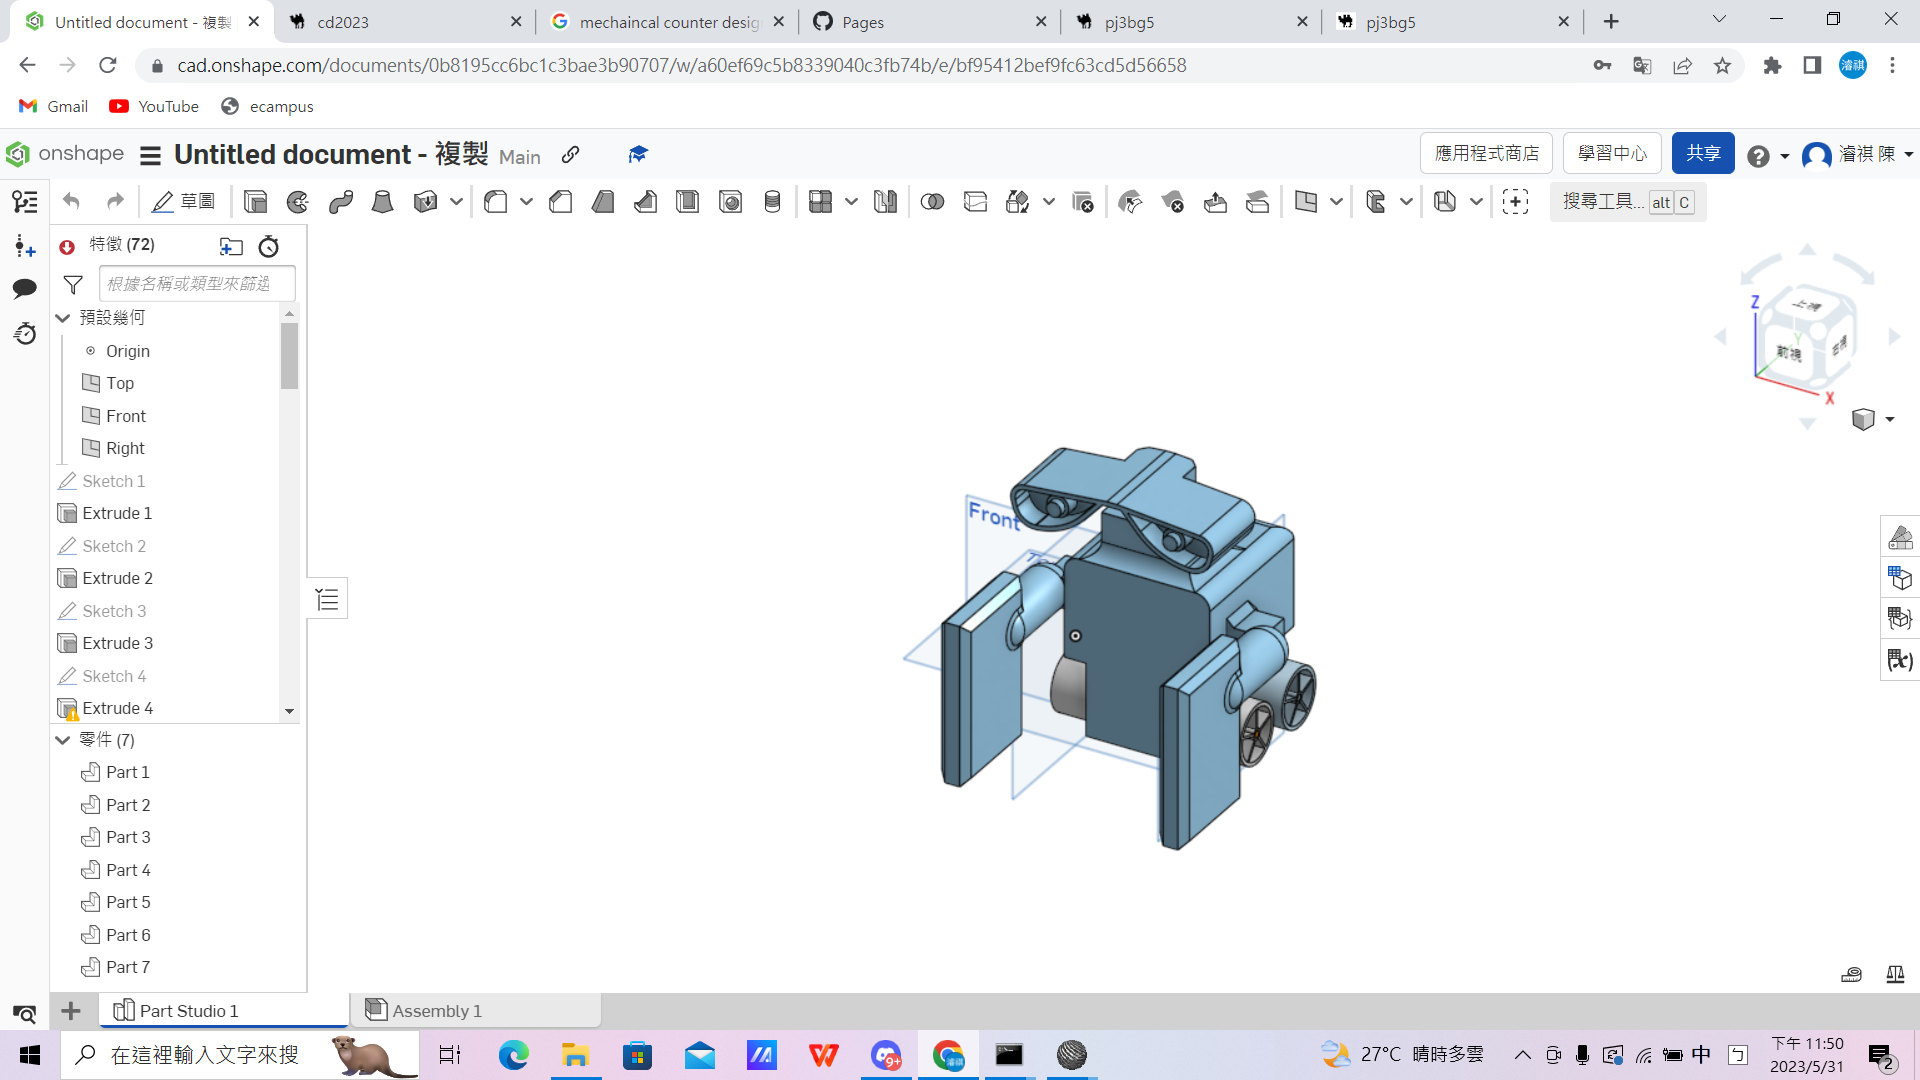
\includegraphics[width=1.25in]{11111}  %作者照片
	\end{figure}
	\end{textblock}}
	{\renewcommand\baselinestretch{0.99}\selectfont %設定以下行距
	{\begin{textblock}{15}(3.5,0.7)%{寬度}(以左上角為原點之右移量,下移量)
	\noindent\fontsize{14pt}{0em}\selectfont \makebox[4em][s]{姓名}\enspace:\enspace
    \fontsize{14pt}{0em}\selectfont \makebox[4em][s]{第一位}\\     \hspace*{\fill} \\
    \fontsize{14pt}{0em}\selectfont \makebox[4em][s]{學號}\enspace:\enspace
    \fontsize{14pt}{0em}\selectfont \makebox[4em][s]{11111} \\ %\makebox為文本盒子
    \hspace*{\fill} \\
    \fontsize{14pt}{0em}\selectfont \makebox[4em][s]{畢業學校}\enspace:\enspace
    \fontsize{14pt}{0em}\selectfont \makebox[9em][s]{國立台灣第一高工}\\
    \fontsize{14pt}{0em}\selectfont \makebox[5em][s]{\quad}\enspace\enspace
    \fontsize{14pt}{0em}\selectfont \makebox[8em][s]{機械工程科}\\
    \hspace*{\fill} \\
    \fontsize{14pt}{0em}\selectfont \makebox[4em][s]{經歷}\enspace:\enspace
    \end{textblock}}}
   % \hspace*{\fill} \\
   \vspace{2em}
	{\begin{textblock}{6}(0,2.3)
	\begin{figure}
	
\includegraphics[width=1.15in]{member2}  %作者照片
    \end{figure}
    \end{textblock}}
    {\renewcommand\baselinestretch{0.99}
    \selectfont %設定以下行距
    {\begin{textblock}{15}(3.5,2.5) %{寬度}(以左上角為原點之右移量,下移量)
\noindent\fontsize{14pt}{0em}\selectfont \makebox[4em][s]{姓名}\enspace:\enspace
\fontsize{14pt}{0em}\selectfont \makebox[4em][s]{第二位}\\ 
\hspace*{\fill} \\
\fontsize{14pt}{0em}\selectfont \makebox[4em][s]{學號}\enspace:\enspace
\noindent\fontsize{14pt}{0em}\selectfont \makebox[4em][s]{11111} \\ 
\hspace*{\fill} \\
\fontsize{14pt}{0em}\selectfont \makebox[4em][s]{畢業學校}\enspace:\enspace
\fontsize{14pt}{0em}\selectfont \makebox[9em][s]{國立台灣第一高工}\\
\fontsize{14pt}{0em}\selectfont \makebox[5em][s]{\quad}\enspace\enspace
\fontsize{14pt}{0em}\selectfont \makebox[8em][s]{機械製圖科}\\
\hspace*{\fill} \\
\fontsize{14pt}{0em}\selectfont \makebox[4em][s]{經歷}\enspace:\enspace
    \end{textblock}}}
    %\hspace*{\fill} \\
    \vspace{2em}
    {\begin{textblock}{6}(0,4.1)
    \begin{figure}
        
\includegraphics[width=1.15in]{member3} %{}內是圖片文件的相對路徑
    \end{figure}
    \end{textblock}}
    {\renewcommand\baselinestretch{0.99}\selectfont %設定以下行距
    {\begin{textblock}{15}(3.5,4.3) %{寬度}(以左上角為原點之右移量,下移量)
\noindent\fontsize{14pt}{0em}\selectfont \makebox[4em][s]{姓名}\enspace:\enspace%\noindent指定首行不進行縮排
\fontsize{14pt}{0em}\selectfont \makebox[4em][s]{第三位}\\ 
\hspace*{\fill} \\
\noindent\fontsize{14pt}{0em}\selectfont \makebox[4em][s]{學號}\enspace:\enspace
\noindent\fontsize{14pt}{0em}\selectfont \makebox[4em][s]{11111} \\ %\makebox為文本盒子
\hspace*{\fill} \\
\noindent\fontsize{14pt}{0em}\selectfont \makebox[4em][s]{畢業學校}\enspace:\enspace
\noindent\fontsize{14pt}{0em}\selectfont \makebox[9em][s]{國立台灣第一高工}\\
\noindent\fontsize{14pt}{0em}\selectfont \makebox[5em][s]{\quad}\enspace\enspace
\noindent\fontsize{14pt}{0em}\selectfont \makebox[8em][s]{機械工程科}\\
\hspace*{\fill} \\
\noindent\fontsize{14pt}{0em}\selectfont \makebox[4em][s]{經歷}\enspace:\enspace
    \end{textblock}}}
   % \hspace*{\fill} \\
   \vspace{2em}
    {\begin{textblock}{6}(0,5.9)
    \begin{figure}
        
\includegraphics[width=1.15in]{member4} %{}內是圖片文件的相對路徑
    \end{figure}
    \end{textblock}}
    {\renewcommand\baselinestretch{0.99}\selectfont %設定以下行距
    {\begin{textblock}{15}(3.5,6.1) %{寬度}(以左上角為原點之右移量,下移量)
\noindent\noindent\fontsize{14pt}{0em}\selectfont \makebox[4em][s]{姓名}\enspace:\enspace
\noindent\fontsize{14pt}{0em}\selectfont \makebox[4em][s]{第四位}\\ \hspace*{\fill} \\
\noindent\fontsize{14pt}{0em}\selectfont \makebox[4em][s]{學號}\enspace:\enspace
\noindent\fontsize{14pt}{0em}\selectfont \makebox[4em][s]{11111} \\ \hspace*{\fill} \\
\noindent\fontsize{14pt}{0em}\selectfont \makebox[4em][s]{畢業學校}\enspace:\enspace
\noindent\fontsize{14pt}{0em}\selectfont \makebox[9em][s]{國立台灣第一高工}\\
\noindent\fontsize{14pt}{0em}\selectfont \makebox[5em][s]{\quad}\enspace\enspace
\noindent\fontsize{14pt}{0em}\selectfont \makebox[8em][s]{機械製圖科}\\
\hspace*{\fill} \\
\noindent\fontsize{14pt}{0em}\selectfont \makebox[4em][s]{經歷}\enspace:\enspace
    \end{textblock}}}
    %\hspace*{\fill} \\
\vspace{2em}
    {\begin{textblock}{6}(0,7.7)
    \begin{figure}
        
\includegraphics[width=1.15in]{member5} %{}內是圖片文件的相對路徑
    \end{figure}
    \end{textblock}}
    \renewcommand\baselinestretch{0.99}\selectfont %設定以下行距
    {\begin{textblock}{15}(3.5,7.9) %{寬度}(以左上角為原點之右移量,下移量)
	\noindent\noindent\fontsize{14pt}{0em}\selectfont \makebox[4em][s]{姓名}\enspace:\enspace
	\noindent\fontsize{14pt}{0em}\selectfont \makebox[4em][s]{第五位}\\ \hspace*{\fill} \\
	\noindent\fontsize{14pt}{0em}\selectfont \makebox[4em][s]{學號}\enspace:\enspace
	\noindent\fontsize{14pt}{0em}\selectfont \makebox[4em][s]{11111} \\ \hspace*{\fill} \\
	\noindent\fontsize{14pt}{0em}\selectfont \makebox[4em][s]{畢業學校}\enspace:\enspace
	\noindent\fontsize{14pt}{0em}\selectfont \makebox[9em][s]{國立台灣第一高工}\\
	\noindent\fontsize{14pt}{0em}\selectfont \makebox[5em][s]{\quad}\enspace\enspace
	\noindent\fontsize{14pt}{0em}\selectfont \makebox[8em][s]{機械工程科}\\
	\hspace*{\fill} \\
	\noindent\fontsize{14pt}{0em}\selectfont \makebox[4em][s]{經歷}\enspace:\enspace
    \end{textblock}}
\newpage
%=----------------書背----------------------=%
\pagestyle{empty}%設定沒有頁眉和頁腳
\begin{center}
\fontsize{0.001pt}{1pt}\selectfont .\\
\vspace{4em}
\fontsize{30pt}{30pt}\selectfont 【13】 \\
\fontsize{20pt}{20pt}\selectfont
\vspace{0.5em}
分\\
類\\
編\\
號\\
\vspace{0.5em}
\hspace{-0.5em}:\\
\vspace{0.5em}
\rotatebox[origin=cc]{270}{\sectionef\LARGE \textbf{112-4-APP-3004-1}}\\ %旋轉
\vspace{0.5em}
網\\
際\\
手\\
足\\
球\\
場\\
景\\
設\\
計\\
\vspace{2em}
一\\
一\\
二\\
級\\

\end{center}
%\newpage
%\begin{landscape}  %橫式環境
%\begin{center}
%\fontsize{0.001pt}{1pt}\selectfont .
%\vspace{70mm}
%\rotatebox[origin=cc]{90}{\LARGE 【14】}\rotatebox[origin=cc]%{180}{\LARGE 1-2-APP-8765} %旋轉
%\end{center}
%\end{landscape}
\end{document}
